% arara: xelatex
% arara: xelatex
% arara: xelatex


% options:
% thesis=B bachelor's thesis
% thesis=M master's thesis
% czech thesis in Czech language
% english thesis in English language
% hidelinks remove colour boxes around hyperlinks

\documentclass[thesis=M,english]{FITthesis}[2019/12/23]

%\usepackage[utf8]{inputenc} % LaTeX source encoded as UTF-8
% \usepackage[latin2]{inputenc} % LaTeX source encoded as ISO-8859-2
% \usepackage[cp1250]{inputenc} % LaTeX source encoded as Windows-1250

% \usepackage{subfig} %subfigures
% \usepackage{amsmath} %advanced maths
% \usepackage{amssymb} %additional math symbols
\usepackage{xevlna, minted}

\usepackage[style=iso-numeric]{biblatex}
\usepackage{todonotes}
\usepackage{longtable}
\usepackage{soul,color}
\usepackage{listings}
\usepackage{xcolor}

\addbibresource{bibliography.bib}


\usepackage{dirtree} %directory tree visualisation
\lstset{basicstyle=\footnotesize\ttfamily,breaklines=true}
\lstset{framextopmargin=50pt,frame=bottomline}
% % list of acronyms
% \usepackage[acronym,nonumberlist,toc,numberedsection=autolabel]{glossaries}
% \iflanguage{czech}{\renewcommand*{\acronymname}{Seznam pou{\v z}it{\' y}ch zkratek}}{}
% \makeglossaries

\definecolor{lightgray}{rgb}{.9,.9,.9}
\definecolor{darkgray}{rgb}{.4,.4,.4}
\definecolor{purple}{rgb}{0.65, 0.12, 0.82}

\lstdefinelanguage{JavaScript}{
  keywords={typeof, new, true, false, catch, function, return, null, catch, switch, var, if, in, while, do, else, case, break, require, assert, emit, let, const, async, await},
  keywordstyle=\color{blue}\bfseries,
  ndkeywords={class, export, boolean, throw, implements, import, this},
  ndkeywordstyle=\color{darkgray}\bfseries,
  identifierstyle=\color{black},
  sensitive=false,
  comment=[l]{//},
  morecomment=[s]{/*}{*/},
  commentstyle=\color{purple}\ttfamily,
  stringstyle=\color{red}\ttfamily,
  morestring=[b]',
  morestring=[b]"
}

\lstset{
   language=JavaScript,
   backgroundcolor=\color{lightgray},
   extendedchars=true,
   basicstyle=\footnotesize\ttfamily,
   showstringspaces=false,
   showspaces=false,
   numbers=left,
   numberstyle=\footnotesize,
   numbersep=9pt,
   tabsize=2,
   breaklines=true,
   showtabs=false,
   captionpos=b
}



% % % % % % % % % % % % % % % % % % % % % % % % % % % % % % 
% EDIT THIS
% % % % % % % % % % % % % % % % % % % % % % % % % % % % % % 

\department{Department of Software Engineering}
\title{Exploring the use of blockchain smart contract in the e-commerce}
\authorGN{Šimon} %author's given name/names
\authorFN{Urbánek} %author's surname
\author{Šimon Urbánek} %author's name without academic degrees
\authorWithDegrees{Bc. Šimon Urbánek} %author's name with academic degrees
\supervisor{Ing. Marek Skotnica}
\acknowledgements{
First of all, I would like to thank my supervisor Ing. Marek Skotnica for his endless patience and instructive advice to this diploma thesis and life. A huge thanks goes to my family who supported me throughout my studies. Last but not least, I thank Bc. Ondrej Pudiš for helping with grammatical and stylistic proofreading of the work. }
\abstractEN{The diploma thesis deals with a use of blockchain technology and its smart contract in the eCommerce sphere. The thesis explains basic concepts to understand blockchain issues in its Ethereum implementation. It places great importance on the analysis of online orders and payments, which is modeled using the BPMP language. Based on the modeled as-is model, a to-be model is created with functional and non-functional requirements and its technological architecture. A decentralized application is created as a proof of concept of the to-be state. The conclusion summarizes the advantages and impacts of using such a model in the real world.}
\abstractCS{Diplomová práca sa zaoberá využitím technológie blockchain a jeho smart contract-u v eCommerce sfére. Práca vysvetľuje základné pojmy k pochopeniu problematiky blockchain-u v jeho Ethereum implementácií. Veľký dôraz kladie na analýzu online objednávky a platby, ktorá je namodelovaná pomocou jazyka BPMP.  Na základe namodelovaného as-is modelu je vytvorený to-be model, funkčné a nefunkčné požiadavky na tento model a jeho technologická architektúra. Ako dôkaz fungovania to-be stavu je vytvorená decentralizovaná aplikácia. Záver práce sumarizuje výhody a dôsledky použitia takéhoto modelu v reálnom svete.}
\placeForDeclarationOfAuthenticity{Prague}
\keywordsCS{technológia blockchain, Ethereum smart contracts, smart contracts in eCommerce, BPNM 2.0, proces online objednávky , smart contract ako sprostredkovateľ transakcii, ochrana spotrebiteľa, návrh softvérového riešenia }
\keywordsEN{blockchain technology, Ethereum smart contracts, smart contracts in eCommerce, BPNM 2.0, online order process, smart contract as a transaction intermediary, consumer protection, software solution design}
\declarationOfAuthenticityOption{4} %select as appropriate, according to the desired license (integer 1-6)
% \website{http://site.example/thesis} %optional thesis URL


\begin{document}

% \newacronym{CVUT}{{\v C}VUT}{{\v C}esk{\' e} vysok{\' e} u{\v c}en{\' i} technick{\' e} v Praze}
% \newacronym{FIT}{FIT}{Fakulta informa{\v c}n{\' i}ch technologi{\' i}}

\setsecnumdepth{part}



\chapter{Introduction}


% Not finished I will finish this after writeng other parts
% Zmieniť data a citácie aby 
% Formálne povedať a definovet, čo chceme chceme vytvoriť
% A definovať ich v bodoch
%
%


Nowadays, we are witnesses to an enormous growth of e-commerce, especially in smaller businesses. A lot of restrictions for in-person selling forced these stores to sell their goods and services online. In this situation, many customers started to ask questions about these new online stores' trustworthiness.

From other point of view, we can hear about fast-growing, almost magical technology called blockchain. Blockchain and its smart contracts has many great use cases. While the most popular is a cryptocurrency, it has an immense potential in e-commerce as well. 

This study deals with a usage of the Ethereum smart contract in an online order process. It is focused on replacing traditional payment intermediaries with public and transparent smart contracts.




\setsecnumdepth{all}
\chapter{Goal}

% Not finished I will finish this after writeng other parts
This study's primary goal is to find a solution for using blockchain and smart contract to raise trustworthiness of new smaller online stores and increase the customers' safety.

This challenge begins with an explanation of the essentials of blockchain technology and its implementation in Ethereum. We present the smart contract and its vision and demonstrate the operation of the transaction and its parameters. We explain terms such as a consensus mechanism, a proof of work and a decentralized application. We also introduce the basics of the BPMN modeling language and its symbols, which will help us later to describe the process.

We will continue by introducing the fundamental pillars of the eCommerce world and its processes, such as payments and delivery. We pay close attention to the purchase contract, which is the legal support for the operation of online orders. At the end of the chapter, we will illustrate the use of smart contracts in eCommerce and select the process for analysis.

The analytical part of the work examines the process of online ordering in detail. We create an as-is model and we describe an order in a state diagram. We also explore various solutions that are already on the market, from which we highlight the importance of buyers' protection in online payments. Based on the collected information, we design a to-be model and define non-functional and functional requirements, which are divided into use cases. Using these requirements, we will produce a technological architecture of the solution.

To verify the functionality of our solution, we create a decentralized application as a proof of concept. A user logs into the application using a crypto wallet and interacts with the created smart contracts. Two smart contracts are created as a backend of the application. The first handles the order logic and the second supports the delivery process. The application is also complemented by tests that show various process transitions.

The conclusion of the thesis looks at the process from a business point of view. It evaluates its advantages and impacts in the real world not only now but also in future.




% This challenge will begin with a proper analysis of the online order process using BPMN process diagrams and a detailed discovery of every element. Based on this knowledge, the solution's architecture will be designed.
% This analysis will prove the solution's concept by using the Ethereum platform and its smart contracts. DasContract software will be used for creating such a smart contract.

% Lastly, it is essential to evaluate the solution from a few perspectives. It will describe the results from cost efficiency and the possibility of future accurate word implementation.

%Firstly, it presents the basic information, terms and definitions required for understanding this study. It provides information about blockchain and its properties and introduces the Ethereum platform and smart contracts.

%Secondly, it analyses the process of online shopping, focusing on payment method with customer protection. It describes today's solutions and the design of the smart contract solution.
%It follows the implementation of the proof of concept of the suggested solution.

%In the end, the thesis summaries the analysed solution from a cost and future perspective.



\chapter{Theoretical background}

This chapter describes the basic theory for understanding this study. The chapter explains blockchain technology, its philosophy and features. Later focuses on Ethereum platform with impressive smart contract technology. At the end of the chapter, the basics of e-commerce and WordPress software with Woocommerce plugin are introduced.

\section{Basic terms} 
\subsection{Peer-to-peer network}
Based on \cite{Schollmeier2002}, a peer-to-peer network is a distributed network architecture, where peers share their hardware resources for providing services or a content between them.
Another, yet not an exact definition is describing peer-to-peer networks as opposite to client-server networks. It is important to realize that there is no intermediary between the peers.
In this document's terminology a peer is addressed as a node in a network.


\subsection{Hash function}

Definition from \cite{CryptographicHash}: \textit{A hash function is a function \texttt{h: D -> R}, where the domain \texttt{D = \{0,1\}*} and \texttt{R = \{0,1\}} n for some \texttt{n >= 1}.}
This definition is not enough for a usable hash function. The essential characteristics of this function are determinism, application to every length of an input, fixed size of the output. Having an input, it is easy and fast to calculate an output, but from the output it is computationally unfeasible to find the input. Also, if we know the input and the output, it is impracticable to find another input with the same output.



\section{Blockchain}

Information provided in this section is from \cite{Nakamoto31October2008} and \cite{Singhal2018}.
% Skôr popísať, čo sa s tým dá robiť, a na čo skúži

Blockchain is a data structure based on blocks, which are cryptographically linked into a chain. A block of data is a group of transactions. Each block has a hash pointer to the previous block (except the first genesis block). The most popular use of blockchain is Bitcoin, which was introduced in 2008 by Satoshi Nakamoto \cite{Nakamoto31October2008}.

The working principle of blockchain is similar in every use case. 
\begin{itemize}
\item It is a peer-to-peer network without third party in between.
\item Every peer has its own copy of the whole chain.
\item It is possible only to insert data into the chain. 
\item No trusted third party is needed for verifying transactions.
\end{itemize}
The block's exact attributes are different in every network. A block of Ethereum will be described later.

\begin{figure}[ht!]
    \centering
    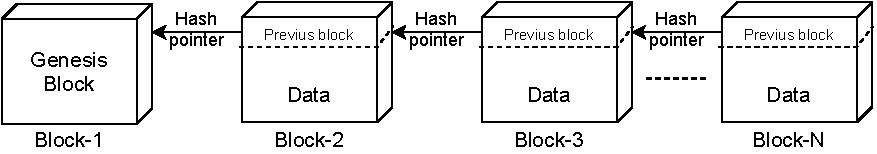
\includegraphics[width=\textwidth]{assets/blockchainidea.pdf}
    \caption{The blockchain data structure \cite{Singhal2018}}
    \label{fig:blockchainidea}
\end{figure}


\subsection{The philosophy of blockchain}

We have described blockchain principles, but how this technology can be used and what the purpose is?  The main goal of blockchain is to create trust between two parties without having a third trusted party.

With reference to \cite{blockchainbusiness}, the point is to avoid the intermediaries, who mediate transactions and maintain integrity, usually for some fee. By replacing this intermediary, we are trying to reduce the transaction fees but keep the integrity. Intermediaries often have the data and services on their own servers, which are vulnerable to crash or be hacked and lose or damage the data. Sometimes we can even dispute about manipulating with our data or sharing our personal information.

Use of blockchain for data management and data authentication is another big topic in this field. We need authority, such as a government, a university, or a certificated organisations, to add their certificates (driving licence, university degree or certification of knowing any skill) to the blockchain. Then we can easily prove our information to another object (for example a new employer). Only we are controlling our personal data.

\subsection{Consensus mechanism}

This section is a sourced from \cite{mediumConsensus}, \cite{ethPow} and \cite{Singhal2018}

The consensus mechanism is an algorithm for creating a consensus (also can be understood in this context as the same state) between nodes in the network. Nodes by this mechanism agree on the current state of the network. It also works as prevention from attacking the network. Theoretically, the attacker has to control majority of nodes to break this algorithm and set their state. The exact percentage relay on a specific consensus algorithm. \cite{ethPow}

\subsubsection{A Proof of work (PoW)}
This algorithm's main idea is that every node has to do a specific amount of work before sending a completed block to the whole network. This work is generally hard to calculate, but easy and quick to verify. In most cases, this work is to solve a cryptographic puzzle, where the only solution is to try and validate every possibility. Example of this cryptographic puzzle is finding a nonce. The nonce is a static-length bit array from which a specific hash is calculated in combination with other data.

This algorithm is running on particular nodes called miners, who are spending their hardware resources. When the fastest miner solves the cryptographic puzzle, they win a reward (usually some amount of coins in the network).
When the network is using the PoW algorithm, as an attacker, one would need 51\% of the network's computational power to defraud the chain. Such an attack would be enormously cost-inefficient and extremely energetically wasteful. In the end, they would lose more than they would get. \cite{Singhal2018}, \cite{ethPow}

\subsubsection{Other algorithms}
We know more consensus algorithms, with specific advantages. In the following section we list a few more of them. 
\begin{description}

\item[Proof of stake (PoS)] is not about mining, it is about validating, instead. The difference is that there is no reward for a winning miner, but the miners are collecting transaction fees. Every validator has to give a deposit as an insurance (or a stake) for validating transactions. If the validator tries to cheat (validate invalid/fake transactions), they will lose their stake in favour of the network. The higher the value of the stake is, the higher the probability of being chosen for validating. Ethereum plans to upgrade to this algorithm. \cite{Singhal2018}, \cite{ethPow}

\item[Proof of Authority] is a mechanism, where only the authorised nodes can validate the transactions. Instead of value as in PoW, they are giving their reputation. This algorithm is suitable for private blockchains. \cite{mediumConsensus}

\item[Practical Byzantine Fault Tolerance] is a broadcast-based algorithm. There are no miners, similar to the PoS, but the working principle is different. Every validator has to validate their part of the final solution, so every validator knows, what others are working on. The final result is based on the majority decision. It is an efficient mechanism compared to others but causes lower anonymity in the network. This protocol is used by Hyperladger, Stellar and Ripple and is famous also in non-blockchain environments. \cite{Singhal2018}

\item[And more]
as Proof of Elapsed Time, Proof of Capacity, Proof of Activity and Proof of Burn.
\end{description}


% Latter after introducing blockchain
%
\subsection{Cryptocurrency Wallet}
A cryptocurrency wallet can be a hardware device, software or a mobile application whose main purpose is to save private keys from cryptocurrency accounts. Next is the list of other standard features of the crypto wallets mentioned in \cite{Suratkar2020928} and \cite{HayNewman11052017}.

 \begin{description}
\item[Signing:]
Most of the wallets also provide other features as signing capability, which is necessary for creating transactions.

\item[Supported currencies:]
Cryptocurrencies which are supported in the concrete wallet.

\item[Key-management:]
We are talking about the place where the keys are stored. Two main categories are non-hosted (only we know, where the keys are) and third-party hosted wallets.

\item[Anonymity:]
We need to consider which information the wallet asks from us. Some wallets don't want any personal information, others want only an e-mail or require a private information set. We need to consider this in case of a hacker attack on the wallet's servers.
\end{description}
Other usual features are converting the coins or tokens, QR code scanner, backup and restoration facility keys.
This thesis works with browser-based wallet Metamask \cite{metamaskWeb}, which supports Ethereum cryptocurrency.

\subsection{Decentralized application}

Decentralized applications or dApps are applications which work on a blockchain in the background. From a user perspective, there is no significant difference from the casual centralized application, but on the backend, they are communicating (not only) with blockchain. They are naturally open-source applications that use user blockchain accounts for login and identification and commonly use blockchain token technology. \cite{dApps}

\section{Smart contract} \label{smartContract}

\textit{``Both the term smart and the term contract are misleading, since a smart contract consists of dumb computer code and rarely represents a legally binding construct."} 
\cite{smartContractBibReview}
 A smart contract is a software script that is living in a blockchain. It is possible to interact with a smart contract thought transactions, which start code execution. The purpose is to create a deal and trust between all involved parties. These values are reached by the transparency of the code, immutability and determinism of the written code. 
 
Smart contract grows up from the idea in Szabo's mind in 1994 \cite{szabo1994} (right, it was before Bitcoin) as a piece of computerized transaction protocol that reduces the need for trust between involved parties. Of course, Bitcoin also supports smart contracts \cite{bitcoinContracts} but only with limited functionality. The first platform to enable fully Turing-complete smart contracts was Ethereum in 2013.

Turing-complete smart contract has many benefits and huge potential but also brings risk in a form of bugs in code. As mentioned before, they can be activated by and only by a transaction. So an external event to fire the execution is needed. The problem is that smart contracts have no information outside of the blockchain (off-chain) and can only react to transactions inside the network (on-chain).
A good way how to understand smart contract functionality is thought examples. Follow a few use-cases of the smart contract.


\begin{description}

%Suppy chain management
%Beef chain management

\item [Hotel room:] Imagine this situation. You want to rent a hotel room. The scenario is following. You choose the room in a hotel, and in front of this room, you unlock the doors by your electronic ID (thought any reader connected to a blockchain, this will represent your digital sign). This act activates the smart contract between you and the hotel. When you finish your stay in the room, you provide your sign in the reader again and then leave the room. The reader sends this act to the smart contract.

Now the smart contract can calculate the price based on the length of your stay, but not only that. The final price calculation can also depend on how much electricity and water you spent (there are sensors for that in the hotel room ). It can also call the cleaning service and finally, charge you. This example was re-written from the original \cite{smartContractBibReview}.

% \item [Mortage example:] This example is based on a case study . At figure  we can see the flow of the smart mortgage contract in DasContract language. It is an excellent example, how smart contract can handle the flow of such a complicated process as the mortgage. Now it is not essential to fully understand every part of this smart contract. The point is to catch visual intuition of what is happening inside, like decision making, computing, changing the property owner, etc. 

%Referencia pridať
\item [Crowdfunding] is an excellent and intuitive example of use. One creates a crowdfunding project with a goal to collect an exact amount of money, and if they find enough backers to reach the goal, they have to realize their project. The project has a time limit. 

In a very simplified version, this smart contract handles three actions. Create a project, back the project and validate. Action create a campaign creates the campaign (obviously). Action back the project saves the backer and adds the backed amount to smart contract account. Validate action checks the campaign's state and determines if the date is after the project's due date. Based on the collected amount it either sends the amount to the creator or returns it back to the backers.

 As mentioned before, a smart contract can't execute this action at the point where the date is equal to the due date because the code can be performed only by a transaction.
 \label{dao}
 \item[DAO] is name of the first implementation of Decentralized Autonomous Organization (DAO) on Ethereum network in 2016 \cite{CHRISTOPH2016}. DAO is a smart contract based organization, which rules and logic are written into the smart contract. The DAO was intended to work as a venture capital fund investing in the crypto. Investors should vote for the investments by DAO tokens, representing the amount of investor's ether (the Ethereum unit) in The DAO. 
 
This project was revolutionary, raising 150 million Dollars in ether at first crowdfunding from 11 000 investors. Everything looked brilliant, but three months after the launch, the DAO was hacked. The code of this smart contract had more problems but was hacked using an exploit at recursive call. The DAO investors lost more than 6O million Dollars in ether. 

This was a massive problem for Ethereum network because this project had around 14\% of all ether. After long discussions, the community of Ethereum decided to hard fork the network, which means that the network's transaction returned in time before this attack happened. Investors had their investments back, but not everyone agreed with this solution. Ethereum network was split into the Ethereum and Ethereum Classic(without the hard fork).

This historical event should teach us, that smarts contract technology is impressive, but when human writes something, there is always a potential threat of bugs. \cite{SamuelDec242017}, \cite{CryptopediaJanuary272021}
 
 
 
\end{description}
\section{Ethereum}
% In this section I am skipping same in formations about Ethereum, witch are not relevant to my work as State, Whole working principle and so on ...


This section was written based on information provided by \cite{ethereumWhitePaper}, \cite{ethereumYellowPaper} and \cite{Singhal2018}.

Ethereum was introduced in 2013 by Vitalik Buterin, as the blockchain platform for building decentralized applications. The goal was not only to fix Bitcoin issues like energy consumption \cite{Baraniuk3July2019} but also to add another possibility for the transactions. Of course, transactions are still supporting cryptocurrency exchange, but help to support even shares, lands, vehicles, online assets and many more.


\subsection{Accounts}

An Ethereum account is used to hold ethers and for signing the transactions. Every account is represented by 20-byte address, which is used for identification and as a reference. An account also has an associated state in the trie (or tree) structure. Ethereum network is tracking the account's state changes. Following information are from \cite{learnEther}.
\begin{description}

\item[Externally owned account (EOA)] is something like a "bank account", and can be controlled using a private key. This key is used for signing transactions. In this account, the structure is only nonce and balance. You can see the structure of EOA in figure \ref{fig:EoAStructure}.

\begin{figure}[ht!]
    \centering
    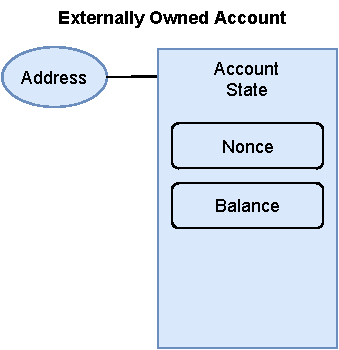
\includegraphics[width=.3\textwidth]{assets/ETHEOAacc.pdf}
    \caption{The blockchain data structure \cite{Singhal2018}}
    \label{fig:EoAStructure}
\end{figure}





\item[Contract accounts (CA)] are controlled only by contained code. The code is called a smart contract as we discussed before in \ref{smartContract}. They are activated only by receiving transactions. The CA account structure consists of nonce, balance, contract code and storage (see figure \ref{fig:CAStructure}).
\end{description}

\begin{figure}[ht!]
    \centering
    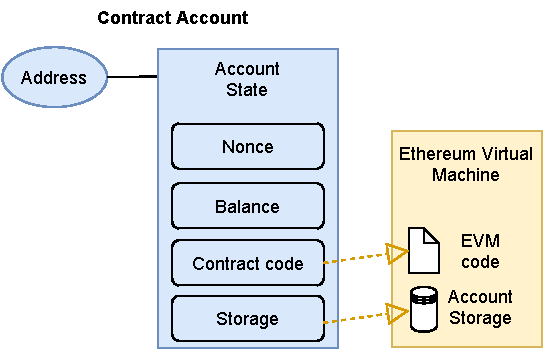
\includegraphics[width=.6\textwidth]{assets/ETHCAacc.pdf}
    \caption{The blockchain data structure \cite{Singhal2018}}
    \label{fig:CAStructure}
\end{figure}

Account data has following attributes.
\begin{description}
\item [Nonce:] 
In EOA account, it is a counter representing a number of signed transactions from account address. 
In CA account, it is also counting the number of created smart contracts.
\item [Balance] shows the current account balance in Wei.
\item [Contract code] is a cryptographic hash of the smart contract's code. If the account type is EOA, this field has an empty string. 
\item [Storage] is a 256-bit cryptographic root hash to Markle tree of account storage. 

\end{description}







%\subsection{Block architecture}

\subsection{Gas and transaction cost}
As mentioned before, Ethereum is a blockchain network powered by cryptocurrency Ether (ETH). Gas in cars is the moving power (with the engine) of the vehicle and similar idea is in the Ethereum. By spending the gas, we are moving from one state of the network to another. We are not buying the gas, we are only paying for gas, that we have used by Ether. 

Ether has smaller units, which are describer in table \ref{EthUnits}. These smaller units exist for two main reasons. Firstly, it is clearer to see how much Wei or more commonly Gwei was spent for executing a transaction than Ether. The second reason is that we can't use double values of prices in transactions, so Ethereum designers made the precision for 18 decimal places (when we pay by Ether). 

\begin{table}[ht!]
\caption{Ethereum Units} \label{EthUnits}
\label{porovnanieDoodleFramadate}
\begin{tabular}{| p{4cm} | p{3cm} | p{5cm} |}
\hline
\textbf{Unit} & \textbf{Wei value} & \textbf{Wei}  \\ \hline
\textbf{Wei}        & 1 Wei     & 1                         \\ \hline
Kwei (babbage)       & \(10^{3}\) Wei    & 1 000                     \\ \hline
Mwei (lovelace)   & \(10^{6}\) Wei    & 1 000 000                 \\ \hline
\textbf{Gwei} (shannon)      & \(10^{9}\) Wei    & 1 000 000 000             \\ \hline
Microether (szabo) & \(10^{12}\) Wei    & 1 000 000 000 000         \\ \hline
Milliether (finney) & \(10^{15}\) Wei    & 1 000 000 000 000 000     \\ \hline
\textbf{Ether} (buterin)      & \(10^{18}\) Wei    & 1 000 000 000 000 000 000 \\ \hline
\end{tabular}
\end{table}

% Gas computation

For every transaction, we need to specify two parameters.
\begin{description}
\item[Gas:] Maximum gas limit to spend for executing the transaction. It is possible to find out the estimated gas for the transaction. It is recommended to set this attribute large enough, because if a transaction does not use all the gas, the unspent gas is returned to sender's account. Otherwise, if the transaction exceeds the gas limit, it is rolled back and gas is not returned. This attribute is also used as a fuse in case of an infinite loop or unexpected exception.
\item[gasPrice:] Is the price for one unit of gas, which the sender is willing to pay. The right price can also be estimated as an average gas price from a previous block or use service info from \url{https://ethgasstation.info}.
\end{description}
The total cost of a transaction is computed as \texttt{gasPrice*gasUsed}, where \texttt{gasPrice} is specified by sender and \texttt{gasUsed} is total gas consumed by Ethereum virtual machine, while processing the transaction. This amount is added to a miner's account as a fee for using their computational resources.

\subsubsection{Cost examples}
In Ethereum blockchain there are two types of transactions. The first type is  a view transaction, which is not changing the state of the network. This transaction does not consume gas. The second type is a gas-consuming but not only for computing but also for storing the data. For better imagination here are examples of gas units used for concrete operations in table \ref{EthGasExamples}. 
\begin{table}[ht!]
\caption{Ethereum operation cost examples}  \label{EthGasExamples}
\label{porovnanieDoodleFramadate}
\begin{tabular}{ll}
\textbf{Operation}                     & \textbf{Approximate gas consuption} \\
ADD - adding two numbers      & 3 gas units                \\
MUL - Multiplying two numbers & 5 gas units                \\
SHA3 hash                     & 30 gas units               \\
Store word "Contract"         & 20 000 gas units           \\
Base transaction fee          & 21 000 gas units           \\
Include 1 MB in transaction data & 68 000 gas units        \\
Store 1 MB of data            &	625 000 000 gas units        \\
\end{tabular}
\end{table}





\subsection{Transactions}

For a better understanding of the analytical part of this thesis, it is essential to have an overview of transaction parameters and requirements and have an idea of what is possible and what is not. Ethereum transaction has a standardized calling structure. Following is an example from web3.js\cite{web3js} library for calling \texttt{sendTransaction(transactionObject [, callback])} function. See the transaction example in \ref{fig:AccountCommunication}. A transaction object has these attributes (simplified):
\begin{description}

\item[from:] Address for the sending account
\item[to:] The destination address. This attribute is undefined, when we are creating smart contract and address is unknown.
\item[value:] Amount of Wei transferred by the transaction.
\item[gas:] Maximum gas limit to spend for executing the transaction. 
\item[gasPrice:] Is a unite price of gas, which a sender is willing to pay. 
\item[data:] The byte string containing the data for a function or smart contract code in case of creating one by the transaction.
\item[nonce:] Nonce of the sending account
\item and more as a chain, hardfork and a common object.
\end{description}

\begin{figure}[ht!]
    \centering
    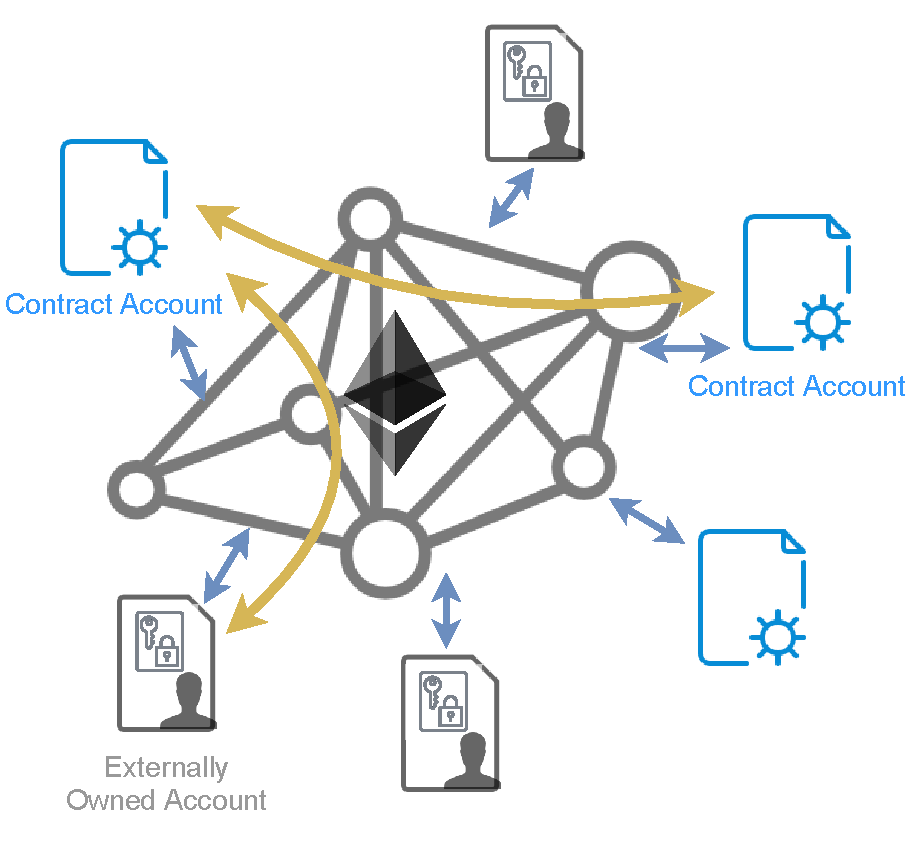
\includegraphics[width=0.8\textwidth]{assets/Accounts.pdf}
    \caption{EOA to CA to CA transaction \cite{Singhal2018} }
    \label{fig:AccountCommunication}
\end{figure}

Every successfully executed transaction is stored in blockchain. Examples of transactions on Ethereum network can be found at \url{https://etherscan.io}. For better imagination, which data are stored, look at the table \ref{etherscanTransactionTable}.

\begin{table}[ht!]
\caption{Ethereum transaction example \cite{etherscanTransaction} }  \label{EthTransactionExample}
\label{etherscanTransactionTable}
\begin{tabular}{| p{0.2\linewidth} | p{0.8\linewidth} |}
\hline
Transaction Hash        & 0x24673cffc87a72730b42dc3ba082f0c03baadd370- 5c95202d4e79e03602e105f \\\hline
Status                  & Success                                                            \\\hline
Block                   & 11868617                                                           \\\hline
Timestamp               & Feb-16-2021 03:19:06 PM +UTC, Confirmed within 11 secs             \\\hline
From                    & 0xa7deccee71c016e76b5af940ceff114b1d28befd                         \\\hline
To                      & 0xf2ce9cee6c632a3cfc54ffa095730f82e318f106                         \\\hline
Value                   & 0.09 Ether (\$161.24)                                              \\\hline
Transaction Fee         & 0.0029001 Ether (\$5.20)                                           \\\hline
Gas Price               & 0.0000001381 Ether (138.1 Gwei)                                    \\\hline
Gas Limit               & 21,000                                                             \\\hline
Gas Used by Transaction & 21,000 (100\%)                                                     \\\hline
Nonce                   & 100                                                                \\\hline
Input Data              & 0x                                                                 \\\hline
\end{tabular}
\end{table}



\subsection{Smart contract in Ethereum}

% Programing Languages

% Structure, Anatomy of smart contract

% optional: Testing, compiling, Deploying

Based on the section about smart contract \ref{smartContract}, we now discuss specifics of Ethereum's implementation of this concept. We can use two new developer-friendly programming languages for creating smart contract.

First language is Solidity which is object oriented programming language influenced by C++, Python and JavaScript \cite{solidityDoc}. It is statically typed, supports inheritance, self-created types and it has a lot of supported libraries. 

The second is Vyper, which is contract-oriented language based on Python. Compared to Solidity, it has fewer features, for example, does not support inheritance, function overloading or modifiers. The reason for not supporting these features is to make it more secure \cite{vyperDoc}. Experienced Ethereum developers can write smart contracts in another language called Yul.

Smart contract consists of functions and data, which are executed in Ethereum virtual machine. Here is a short overview of what we can use in smart contract Ethereum programming.
\begin{description}

\item[Data] are divided into three sections: storage, memory and stack. Storage data are stored in blockchain forever. They are representing the state of a smart contract. They support large scale of types from booleans, integers and strings to enums or custom-made types. Memory data are living only in function and then they are discarded. They are cheaper to use because we are not spending gas for storing them. It is possible to use global variables mostly for getting information about the current transaction (who is the sender) or block information.\cite{RichardsJanuary202021}
\item[Functions] can be divided into two types based on call. When we communicate with a smart contract we are calling external functions. All external functions are part of the contract interface. An internal function can be called only from a smart contract itself. We can also talk about private and public function. The difference is that public functions can be called internally or externally but private only from inside the contract, where they are defined.

An important term is a view function. The specific of this function is that it is not changing the state of the contract. It is only providing a view inside, commonly to get the storage data.
 
Events are a special construct which work as publisher-subscriber pattern. When a specified event is triggered inside the contract, this event will provide its information to the subscribers, usually a frontend application.\cite{RichardsJanuary202021}
\end{description}



\section{BPMN}

Following section is based on \cite{quickBPNMguide} and supported by \cite{manualBPNM}. Business process modelling and notation is a language that provides a wide range of symbols and signs, that are highly intuitive and easy to understand even for non-specialists. Symbols are divided into activities, gateways, events, flows, swimlanes, artefacts and data. 

We will later use this notation to create a well-understood as-is and to-be models of the observed process. According to \cite{fundementalsBPNM} as-is model describes a current state of the process. This model is created based on process identification, process documentation, and possibly based on process metrics. On the other hand, a to-be model describes the process in future. It is often based on the as-is model in which the changes were proposed.

Model of one process can have more BPMN models based on a chosen level of abstraction. For high-level overview (typically for business persons) complicated structures and advanced symbols are not used . We can also talk about executive models for BPMN systems, which can execute the modelled process. In this case, BPMN components are chosen for supporting the concrete system. Some systems are not supporting every symbol, and models can have slightly different behaviour in each software. Another type of BPMN modelling style is not to create executable models but informative models. These models have a purpose of explaining the process, usually with specialization (on data/information flow, process chaining etc.). Now follows a quick overview of BPMN essentials.

\subsection{Activity}
An activity indicates a general concept of work in a certain process. The activity is commonly atomic, i.e. it is no longer divided to lower levels of detail. If the activity is not atomic, we speak of a non-atomic activity called a thread. The thread must be marked with a special symbol (Table \ref{tableAktivity}, line 2). The activity becomes more specific by adding additional markings to the upper left side or the middle-lower part (Table \ref{tableAktivity}, line 4) of the rectangle. The activity may have a participant defined by a pool, and a swimline assigned. Selected types of assets are listed in table \ref{tableAktivity}.

\begin{table}[ht!]
\caption{Activity} \label{tableAktivity}
\begin{center}
\begin{tabular}{ | p{1cm} | m{9cm} | } \hline
    
\includegraphics[width=1cm]{assets/BPNMicons/abstractActivity.pdf}     & We note abstract activity by a rounded rectangle. 
 \\   \hline
    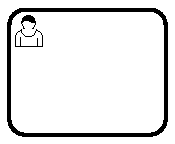
\includegraphics[width=1cm]{assets/BPNMicons/UserActivity.pdf} & User task is the work that a person does using a software application.  \\  \hline
    
\includegraphics[width=1cm]{assets/BPNMicons/ManualnaUloha.pdf} & A manual task is a job performed by a person without software or other supporting equipment.  \\ \hline
    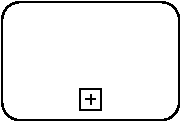
\includegraphics[width=1cm]{assets/BPNMicons/Podproces.pdf} & A thread is an activity that encapsulates a process. The context of this process is either irrelevant or explained in a separate diagram.  \\ \hline
\end{tabular}
\end{center}
\end{table}




\subsection{Gate}

A gate is used to control the flow in a process. The gateway supports multiple inputs and outputs, allowing it to marge or split flows. We can divide flows using conditions, signals, events or our own rules. This behaviour is giving a lot of flexibility to the model. If it is not necessary to control the flow in the process, we do not need gateways. Selected types of gates are listed in table \ref{tableGate}.



\begin{table}[ht!]
\caption{Gates} \label{tableGate}
\begin{center}
\begin{tabular}{ | p{1cm} | m{9cm} | } \hline
    
\includegraphics[width=1cm]{assets/BPNMicons/ExkluzivnaBrana.pdf} & Exclusive gateway: When merging, it is sufficient if one stream arrives and the exclusive gateway passes the flow further.
When splitting, the exclusive gateway passes just one flow.  \\   \hline
    
\includegraphics[width=1cm]{assets/BPNMicons/InkluzivnaBrana.pdf} &  
Inclusive gateway: When merging, the flow must be active from all incoming branches to allow the flow to continue.
When splitting, it can allow flow through multiple branches.   \\  \hline
    
\includegraphics[width=1cm]{assets/BPNMicons/ParalernaBrana.pdf} & Parallel gate: When merging, the flow must be active from all incoming branches to allow the flow to continue.
When divided, it lets flow through all branches.  \\ \hline
    
\includegraphics[width=1cm]{assets/BPNMicons/KomplexnaBrana.pdf} & Complex Gateway: Merging and splitting is defined by the gateway's own rules provided by the comment. \\ \hline
    
\includegraphics[width=1cm]{assets/BPNMicons/BranaNaZakladeUdalosti.pdf} & Event-based gateway: The branches that exit the gateway have events assigned to them and are triggered depending on those events.  \\ \hline
\end{tabular}
\end{center}
\end{table}


\subsection{Event}

An event is a construct, which occurs during a process. These events can affect the flow of the process and usually have some trigger or impact (result), based on its type. We can see events as circles with written marks in the middle. Based on the impact on the process, we recognize three types of events, namely start, intermediate, and end. All start events and some intermediate events can capture facts from the process what cause start flow from them. We can call them pending events that are waiting to run. Some intermediate and all ending events throw a fact as a result, which can turn into an event that another pending event can capture. Selected types of events are listed in table \ref{tableEvent}.



\begin{table}[ht!]
\caption{Events} \label{tableEvent}
\begin{center}
\begin{tabular}{ | p{1cm} | m{9cm} | } \hline
    
\includegraphics[width=1cm]{assets/BPNMicons/PraznaStartovaciaUdalost.pdf} & An empty start event does not need to have a trigger defined. It starts at the beginning of the process. \\   \hline
    
\includegraphics[width=1cm]{assets/BPNMicons/PrazdnaKoncovaUdalost.pdf} & An empty ending event has no result. This event is used to end the flow.  \\  \hline
    
\includegraphics[width=1cm]{assets/BPNMicons/PrazdnaMedzilahlaUdalost.pdf} & 
An empty intermediate event is used only in the classic process flow. Even if it does not have a trigger defined, it has a defined result. Used to model those events that determine a change in process state.  \\ \hline
    
\includegraphics[width=1cm]{assets/BPNMicons/messageThrow.pdf} & Throw - message intermediate event sends a message toward the capture event, shifting the flow.\\ \hline
    
\includegraphics[width=1cm]{assets/BPNMicons/messageCatch.pdf} & Catch - Message intermediate event is an intermediate event. This event triggers a flow when it receives a message.  \\ \hline
\end{tabular}
\end{center}
\end{table}


\subsection{Flow}

The activities, gates and events are connected by connecting objects. These objects are used to show the direction of the flow of a process or to assign two objects to each other. In general, a connecting object is a line (solid, dashed, dotted) or a different type of an arrow. In case of an arrow, the tip of the arrow determines the flow direction or the direction of the association. Symbols may appear on the line that adjusts the flow behaviour. Selected types of flows are listed in table \ref{tableFlow}.


\begin{table}[ht!]
\caption{Flows and association} \label{tableFlow}
\begin{center}
\begin{tabular}{ | p{2cm} | m{9cm} | } \hline
    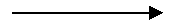
\includegraphics[width=2cm]{assets/BPNMicons/SekvencnyTok.pdf} & Sequential flow is used to display the order of activities that will be performed in the process. \\   \hline
    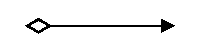
\includegraphics[width=2cm]{assets/BPNMicons/PodmienenyTok.pdf} & Sequential flow can have a condition that determines flow through a given branch. Such a sequential flow is called a conditional sequential flow and is used when the flow is based on activity.   \\  \hline
    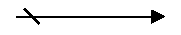
\includegraphics[width=2cm]{assets/BPNMicons/StandartnyTok.pdf} & For exclusive or inclusive gates, one type of branch can be referred to as a standard flow. The flow will go through this branch only if it is not possible to go through any other. \\ \hline
    
\includegraphics[width=2cm]{assets/BPNMicons/TokPreSpravy.pdf} & The message flow is used to deliver messages between two roles that are ready to receive or send them.   \\ \hline
    
\includegraphics[width=2cm]{assets/BPNMicons/AsociaciaDat.pdf} & A data association is a subspecies of an association and focuses on retrieving, transmitting, and storing data with a specific data store.   \\  \hline
\end{tabular}
\end{center}
\end{table}

\subsection{Artifacts}

Artifacts are used primarily to refine information and bring greater detail from the process. Selected types of artifacts are listed in table \ref{tableArtefakt}.


\begin{table}[ht!]
\caption{Artifacts} \label{tableArtefakt}
\begin{center}
\begin{tabular}{ | p{1cm} | m{8cm} | } \hline
    
\includegraphics[width=1cm]{assets/BPNMicons/Skupina.pdf} & A group of graphic elements that expresses a common property of activities. I give activities to groups for analytical or documentary reasons. \\   \hline
    
\includegraphics[width=1cm]{assets/BPNMicons/Komentar.pdf} &A text commentary is a way to add additional information to a chart reader.  \\ \hline
\end{tabular}
\end{center}
\end{table}




\subsection{Pool and swimlane}
Pools are showing responsibilities for activities. The pool can be divided into lanes to show mode details, especially to divide entities and organizations, based on the use case. Pools and swimlanes are explained in table \ref{tablePool}.

\begin{table}[ht!]
\caption{Pool and swimlanes} \label{tablePool}
\begin{center}
\begin{tabular}{ | p{3cm} | m{8cm} | } \hline
    
\includegraphics[width=3cm]{assets/BPNMicons/Bazen.pdf} & The pool is a graphic representation of the entity. The pool supports the overall layout, so it can be divided into smaller and more detailed parts using lanes. When the pool does not contain internal information about the processing of the process, we speak about a "black box" pool. \\   \hline
    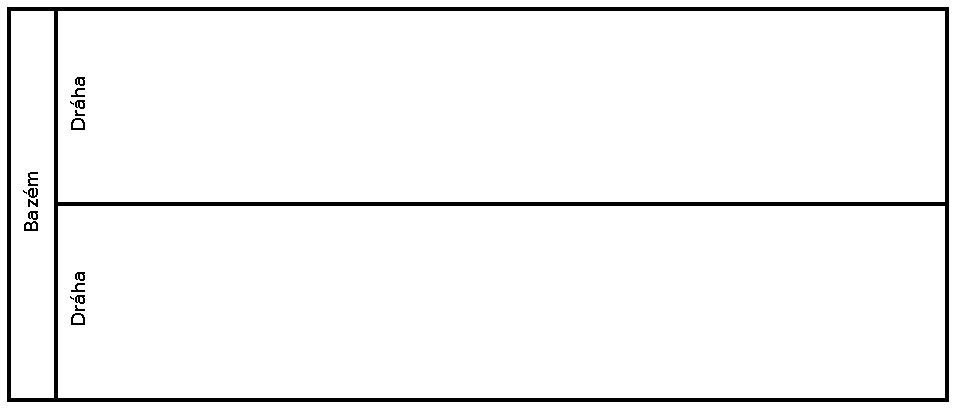
\includegraphics[width=3cm]{assets/BPNMicons/Draha.pdf} & The lanes are used to organize and categorize activities.  \\ \hline
\end{tabular}
\end{center}
\end{table}


\subsection{Data}
Data objects have the purpose of transferring information between activities. The selected data objects are described in table \ref{tableData}.

\begin{table}[ht!]
\caption{Data objects} \label{tableData}
\begin{center}
\begin{tabular}{ | p{1cm} | m{8cm} | } \hline
    
\includegraphics[width=1cm]{assets/BPNMicons/dataObject.pdf} & The data object serves as a variable in the process that carries the information. At the end of the process, the data object is lost. \\   \hline
    
\includegraphics[width=1cm]{assets/BPNMicons/databaseobject.pdf} & The data storage serves similarly to the object for transmitting information, with the difference that after the end of the process, this data is stored.  \\ \hline
\end{tabular}
\end{center}
\end{table}


%  DEMO sa už nepoužíva


\section{Das contract}
This section is written based on \cite{dasContract} and \cite{newDasContract}.
We have discussed smart contracts and BPMN, and now its time to put it together. Das Contract is a "formal language that use BPMN models to describe a smart contract with high conceptual quality and enough expressiveness to contract between people."\cite{dasContract}

The best way how to understand Das Contract is to look at why it was created. A contract was written on a paper or only spoken between people before the digital age. In this type of communication, there was room for misunderstanding or misinterpretation of the contract between parties. On the opposite side, there are smart contracts with zero tolerance for non-specified facts because they are written in immutable code. That sounds great but is unreadable for a person who does not understand the specific programming language (it is sometimes hard even for programmers). Also, as we mentioned before in \ref{dao}, in a smart contract written by a human, there can be bugs, which can cause a catastrophic scenario.

Das Contract offers a solution in form of advantages from both sides. From the classical paper form, we have a strict fact and no place for misunderstanding the contract, and visual and well-described support for understanding the process and rules.
We will use Das Contract as a methodology for creating smart contracts. The speciality of processes created by this methodology is a timer. We can't implement an accurate timer or a cron function in smart contracts (the code can be executed only by transaction). So we use a skip function which anyone can call with an intention to change the state of the process. We also use the Das Contract data model for describing data inside the system.


\chapter{Smart contract in eCommerce}

This chapter is an introduction to the basic aspects of the eCommerce world. It covers the problems of eCommerce technical solution and basic elements of eCommerce business. It provides information about product restrictions and online selling problematic as purchase contract. It also covers the most famous payments methods and delivery methods. At the end, we will talk about use of block chain and smart contract in payments, supply chain, reviews and marketing.


\section{Technical solutions}
When you want to start selling online, you need some platform or a solution. The right solution depends on your individual needs, the number of products you want to sell and on your budget. Now follows a list of four possible ways divided by the technical complexity of the solution.

\begin{description}

\item[Online market (marketplace):] This is the simplest way to start selling goods online. You are selling on domains of the chosen market and the marketplace solves all critical problems such as the infrastructure of the store and trusted payments. You focus on your product and marketing around it. Most of this solution has a service called buyer protection and if a customer is unsatisfied with the product, they can open a dispute and want a refund. In this case, the marketplace acts as a judge between you and the customer. 
The disadvantage of this marketplace is that they are highly product-oriented and you don't have many opportunities to present your brand and low customizability of product page.
The famous representatives by \cite{similarWebMarketplace} of this category on global market are Amazon, E-bay and Aliexpress.

\item[SAAS Solution:] System as a service solution is providing pre-programmed store software. Commonly you have your own domain with a chosen design template customized to your brand identity. The level of customization is limited because you are not able to change the code. This solution comes with a pre-integrated payment solution, and in most cases, there is no possibility to add a non-supported payment gateway. You are paying a monthly fee for renting the software.
The company representatives are Shopify and Shoptet.

\item[Free/Paid customizable solution:]
Similarly, as in the SAAS solution, there is a pre-programmed store software, but we need to install it on our own server. Selling is provided on the seller's domain address. Many of these solutions offer pre-made design templates which are ready to customize to seller's brand. They are usually more customizable than the SAAS solutions or pre-made elements are used. These solutions are based on plugins where external developers can expand the basic functionality of the system. They are mostly paid, but creating a custom plugin to support third-party payment solutions is possible.
This solution is a compromise between SAAS and a custom made solution.
General examples are WordPress with Woocommerce and PrestaShop.

\item[Custom made solution:] 
There is no concrete description for this solution. Basically, the possibilities are limited only by the used technology. Everything is customizable, but requires a programming skill which is not cheap in these times. This solution is reasonable for a big project with a significant budget.

\end{description}


\section{Products}

% Identification of the products


Two basic categories of products are services (also tickets for events, flights) and goods (can be non-physical as software). This thesis is focused on selling goods and we will also specify the attributes of these goods. 
By selling the products, we are often dealing with a restriction of selling. The common restrictions are:
\begin{description}
\item[Age restrictions:] Best examples are alcoholic beverages or tobacco products.
\item[Location legality restrictions:] Some products can be illegal in certain locations.
\item[Licence restriction:]For buying product as guns or medicaments.
\item[Shipping restrictions:] Some products cannot be shipped or special shipping method is needed. Examples are animals or hazardous materials.
\end{description}
It is the seller's responsibility to check if these restrictions are not broken. For example, the delivery person can check the buyer's age or an ID needs to be provided to the seller.

\label{purchaseContract}
\subsection{Purchase contract}
The critical topic in eCommerce is the purchase contract signed at a distance. This is a specific type of contract with particular rules. This thesis does not have enough space to discuss all law specifics, so it describes only parts needed to understand the problematic. The next pieces of information is from Slovak law codex 102/2014 \cite{customerProtection} and is neither word to word nor officially translated.

The fact why this type of purchase contract is important is that the customer has a right to withdraw from the contract up to 14 days from acceptance of goods (law documents contain more cases, but the ones listed below are relevant in this study). The goods are considered to have been taken over by the consumer at the moment when the consumer or a third party delegated by them, with the exception of the carrier, takes over all parts of the ordered goods, or if
\begin{itemize}
\item the goods ordered by the consumer in one order shall be delivered separately, at the moment of taking over the goods, which were delivered as last,
\item delivered goods consist of several parts or pieces, at the moment of taking over the last part or the last piece.
\end{itemize}
This law document describes twelve exceptions when the customer cannot withdraw from the purchase contract. Relevant for this study are
\begin{itemize}
\item the sale of goods made to the consumer's special requirements, custom-made goods or goods intended specifically for one consumer,
\item the sale of goods which are subject to rapid deterioration,
\item the sale of goods enclosed in protective packaging which cannot be returned for health or hygiene reasons and whose protective packaging has been broken after delivery,
\item the sale of sound recordings, video recordings or computer software sold in protective packaging, if the consumer has unpacked that packaging.
\end{itemize}

The responsibility of proving the application of the right of withdrawal lies on the customer. They are obliged to send the goods back or hand them over to the seller or a person authorized by the seller to take over the goods no later than 14 days from the date of withdrawal from the contract. This does not apply if the seller proposes to pick up the goods in person or through a person authorized by them. The time limit referred to in the first sentence shall be deemed to have been observed, if the goods were handed over for transport no later than the last day of the time limit.

Upon withdrawal from the contract, the consumer bears only the cost of returning the goods to the seller or the person authorized by the seller to take over the goods. This does not apply if the seller has agreed to bear them themselves or if they have not fulfilled the notification obligation mentioned above.

The consumer is only liable for reduced value of the goods that have arisen due to such treatment of the goods as it is beyond the scope of the treatment necessary to ascertain the characteristics and functionality of the goods. The consumer is not responsible for the reduction in the value of the goods if the seller has not fulfilled the obligation to provide information on the consumer's right to withdraw from the contract.

In addition to the obligations mentioned above, it must not give rise to additional costs or other obligations for the consumer.

The seller is obliged without undue delay, no later than 14 days from the date of delivery of the notice of withdrawal to the consumer to return to the consumer all payments received from them under or in connection with the contract, including transport, delivery and postage and other costs and fees.

The seller is not obliged to reimburse the consumer for additional costs if the consumer has explicitly chosen a method of delivery other than the cheapest standard method of delivery offered by the seller. Additional costs are the difference between the consumer's delivery costs and the costs of the cheapest delivery method offered by the seller.

Upon withdrawal from the contract for the sale of goods, the seller shall not be obliged to reimburse the consumer for payment before the goods have been delivered to them or until the consumer proves good's return to the seller. Unless the seller proposes to pick up the goods in person or through them authorized person.

The store also has the right to cancel the order, especially for the following reasons:
\begin{itemize}
\item if it is not possible for technical reasons to deliver the goods within the required period or under the conditions of the order,
\item if the goods are no longer manufactured or delivered or their price charged by the supplier of the goods has changed significantly.
\end{itemize}
Other reasons for withdrawal from the contract may be specified in their terms and conditions.

\label{paymentmethods}
\section{Payments}

At this time, we recognise a lot of various online payment methods. Each of them has its advantages and disadvantages. Below find a quick overview of the most used online payment methods by \cite{statistaPaymentMethods} in 2019 and a few more. See figure \ref{fig:StatistaPaymnentsMethods}.

\begin{figure}[ht!]
    \centering
    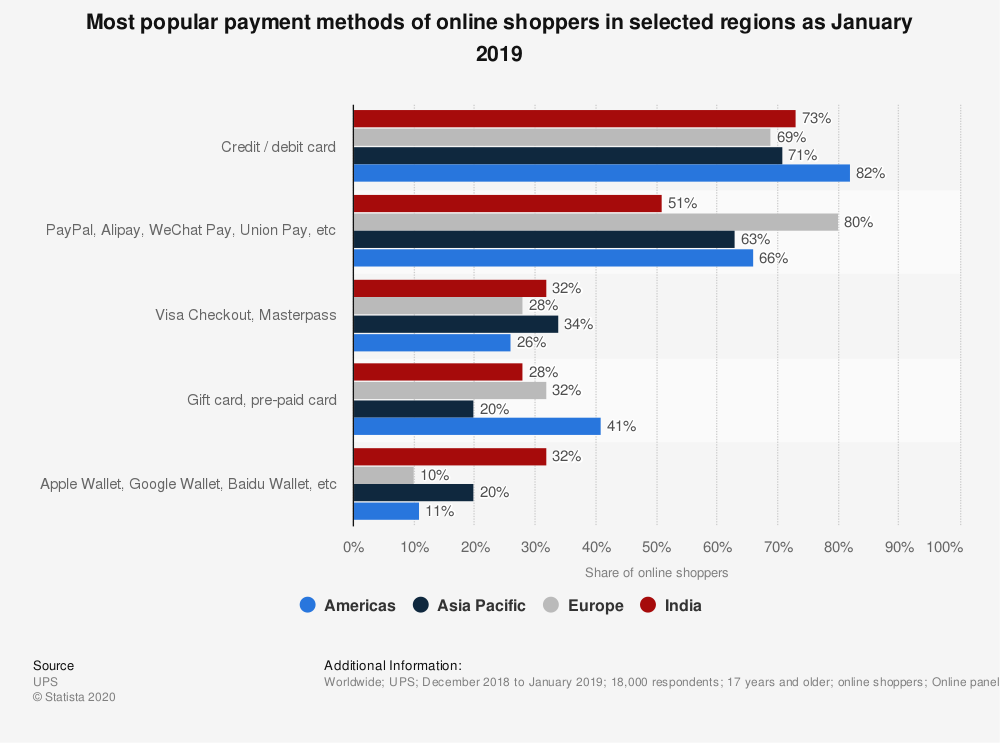
\includegraphics[width=\textwidth]{assets/statistic_id676385_preferred-online-retail-payment-methods-worldwide-2019-by-region.png}
    \caption{Most popular payment methods of online shoppers in selected regions as January 2019}
    \label{fig:StatistaPaymnentsMethods}
\end{figure}



\begin{description}

\item[Credit/debit cards:]
In this payment method, the payer provides card details information to the merchant or directly to the payment gateway. Then payment gateway continues through the payment processor to the right card network and then to the card issuer.
In case of a problem with the purchased item (it is not delivered, wrong goods are delivered and so on), the card issuer takes care of the payment and can start the goods claim process. In this process, the card issuer asks for evidence of communication with a store and all recipes from the store and optionally the photos of delivered goods. The issuer is taking these steps when the store is not answering or when the customer can't contact the store in any way. In case of a problem, the recommended way of communication is a registered letter or an official store email. In case the customer is right, the card issuer can execute a chargeback of the payment. \cite{creditCardInfo} \cite{tatraBank}

\item[Paypal, Alipay, WeChat pay:]

In this case, the customer is paying thought intermediatory. The payment is not going directly to the store account but to the intermediatory account and later is sent to the store. And this is a huge advantage of the payment solution. When a problem appears, the money is not directly at the store's account, so the intermediary can hold it until the problem is solved. The intermediary often has the position of "a judge" in problematic situations when the purchase is not in the local law's competence. This solution is discussed deeply in section \ref{existingSolutions}.

\item[Visa Checkout, Masterpass:]
These solutions are nowadays merged together as click to pay services. In short, the customer has an account where they store their credit/debit cards, and can make a purchase on the stores where the click to pay functionality is integrated. \cite{clickToPay}
% https://www.merchantmaverick.com/click-to-pay/ 
% Charge back 


\item[Apple pay, Google wallet:]
These solutions also work on storing the card details and then providing the interface for paying. The difference is that customer can use this solution also in offline paying mode thought a payment terminal. These services are not intermediaries in the right way because they are not storing any money. They are only providing the bridge for direct transfer. In case of problems, the customer has to contact the card issuer.

\item[Cash on delivery:]
It is an offline payment method, but it is needed to mention it here because it is one of the classic payment methods. 

\item[Internet banking:]
Direct money transfer to the store's account. The recognising key for merging payment is the variable symbol, which is the number of the order. 

\item [Crypto:]
Crypto payments work similarly to direct bank account transfers. Some solutions work on the market as an intermediatory as Utrust \cite{utrust}, but they are mostly in a prototype stage. There is no standardized solution, how to pay safely for goods.
 
Furthermore, when you are scammed and you use crypto payment, there is no bank chargeback possible. The customer is fully responsible for their signed transactions.
\end{description}



\label{deliveryMethods}
\section{Delivery}
Delivery is a fundamental part of the shopping process, which can significantly affect the customer's final satisfaction. Next are the basic types of delivery methods with their typical use cases.
\begin{description}

\item[Courier delivery:] One of the most typical delivery method. The delivery person comes to the customer's house and gives them (or the delegated person) ordered goods. Depending on the specific delivery type and implementation of the company, the delivery person can make an act of security check (ask for a code sent to them via SMS or e-mail) or ask for a signature of receiving person (and ID in some cases). This act is marked in this thesis as a confirmation mechanism because it simply proves that an authorised receiver took the goods. It is necessary to mention that this confirmation mechanism is not mandatory, and it does not happen in all courier delivery cases, which may cause significant problems. On the other hand, it is cheaper and more time-efficient for the delivery company. The delivery person only leaves goods at the selected address.
Various kinds of shops use this delivery method.

\item[Post packet:] Postman delivers products at the address (usually without confirmation mechanism), or the customer has to go to the post office and pick up the goods in person.

\item[Local delivery:] This is a typical delivery used by food stores or restaurants, which has to be quick. This delivery is provided by a local delivery service or in house (imagine pizza delivery). 

\item[In house delivery system:] It is commonly offered by larger online stores but is not a rule. The store has its deliverer or uses special post boxes with an authentification of the withdrawer. 

\item[Withdraw point:]  Following the previous point, the withdraw points are also a kind of an authorised service. The withdraw point doesn't have to necessarily be an in-house solution. \cite{zasielkovna}

\item[Others:] As mentioned before, some goods need special delivery. Representative examples are furniture, animals or trees. 
\end{description}


%  \subsection{Law}

%  \subsubsection{GDPR and privacy}

%  \subsubsection{Law changes}


%  \subsection{WordPress}

%  \subsection{Woocommerce}

\section{Blockchain in e-commerce} \label{blockchainInEcommerce}


This section is a review of usage of blockchain and smart contracts in the eCommerce sphere. We discuss possible applications of this technology, and for some cases, we introduce real projects and software solutions. We also mention a few examples of smart contract usage in \ref{smartContract}, so this section digs deeper and merges technology which a sector of natural application.


\subsection{Payment methods}
Everyone knows the famous button pay by "something" as Pay by credit card, Pay by Paypal, Pay by Bitcoin etc. Thanks to blockchain's immutable character, it suits well for providing a trusted payment mechanism and you would rather choose Pay by Ethereum protected by smart contract than Paypal. This thesis describes this payment process more deeply in the next chapter \ref{existingSolutions}.

\subsection{Supply chain management}
Supply chain management is a promising field of use of blockchain technology and it is a massive topic in eCommerce. The idea of using a smart contract as an intermediary and a single source of truth will connect parties involved in the supply process in an immutable master ledger. It can create a relationship not only between business parties but also between the seller and end customer. 

\begin{description}

\item[Support for supply delivery:]
The primary goals for using the smart contract in this process are to increase transparency, improve traceability and higher efficiency. As for example, imagine an online shop with custom PC builds. When a customer makes an order for a custom PC build a smart contract can check the actual prices of a certain component and then order the chosen one based on specific criteria. The deliverers see their orders and, based on the contract, can specify the delivery method and delivery date. This smart contract can also manage the logistics and assume the production date for the final product. What is truly impressive is that this process can be easily chained. One contract makes an order from another, and then the second makes an order based on the original order and so on. In our PC example, a motherboard producer can order a SSD which will be built into this board. This small example does not directly show the big advantages of this solution but imagine the car industry process, with hundreds of suppliers.\cite{Angwei2017}

\item[Tractability for end-user]
The traceability of the product prevents the customer from buying fake products and increases the seller's trustworthiness.  It is a big topic, specifically in the food industry, where we can find already successful projects as Beef chain\cite{beefChain} or Smucker’s Folgers coffee farms\cite{CoffeeChain}. Customers or consumers can see the whole distribution process, from where the product was grown or manufactured to how the delivery company transferred it to their seller. Simply they can discover the history of the product.
\end{description}


An excellent example is wowtrace.io\cite{wowtrace} which is a traceability solution for businesses. The end-user can simply scan a QR code and see the details about the product. As an example, they provide an orange history, from growing place and farm, thought harvesting to distribution to a local store. The example also provides information about expiration dates, producers and certificates.

The food industry is not the only example of the importance of trusted traceability. The pharmacy, fast-moving consumer goods or luxury product industries are other adepts for high level transparency and traceability. \cite{healthcareBlockChain} informs about four ways how blockchain and smart contract can significantly improve the healthcare industry and build a genuine end-to-end supply chain. The topics are drug quality and security act, controlled substance monitoring, cold chain monitoring and ending with active pharmaceutical ingredients. If we merge these ideas with online drug selling, the use is even more critical.

\subsection{Genuine reviews}
\emph{"92\% of 18-34-year-olds have read a fake review in the last year" }
says \cite{brightLocalStat} from their \cite{brightLocalSurway} survey from 2020 which is an enormous number. The problem with good or bad fake reviews is truly hard to imagine. Another interesting statistic from \cite{qualtrics} is \emph{" 91\% of 18-34 year olds trust online reviews as much as personal recommendations, and 93\% of consumers say that online reviews influenced their purchase decisions."}

When we put it together, it makes an enormous mistrusted and misleading information scope. In the analytical part, we talk about reviews on Google, Facebook and Heureka more, with details about how they authenticate the review and how the businesses can defend themselves. What do all these have in common with blockchain and smart contract? It can't solve the situation itself, but connected with orders, products, and services thought smart contract could be easily validated if the user really used reviewed service. 

\subsection{Fraud reduction}
Fraud reduction is not a use, but an effect of using the blockchain. Based on \cite{fraud}, the eCommerce businesses lost more than 57 billion dollars by frauds. If we use a smart contract, it doesn't mean that the fraud and scammer stores disappear, but they will have more challenging work again. If people use a button to pay by crypto protected by a smart contract, it actually does not mean anything. Same as with Paypal, the redirection doesn't have to be on Paypal's webs, and if the customer is not careful enough, they can be easily cheated.

Nowadays, customers are (thankfully) harder to cheat, and if they are not feeling secure enough, they leave the web instead of taking a risk. It will require teaching the users how to check if they are using the right smart contract for their purchase protection or a nice new feature or cryptocurrency wallet. As browsers warn us that we are on a non-trusted web, the wallets can warn us that we are using a non-authorised smart contract.





    
\subsection{Marketing}
Marketing is an essential part of each online store. It is a summary of activities which purpose is to bring potential customers to the store and encourage former customers to purchase. In order to achieve this goal, online stores use various tools and platforms for advertising. But how can blockchain and smart contract change marketing?

According to Campbell R. Harvey from the National Bureau of Economic Research in Cambridge \cite{blockChainMarketing}, blockchain will change the whole marketing industry. We mention a few of his ideas and add theoretical implementation example for them.

The first brave idea is that blockchain will end Google's and Facebook's duopoly in the digital advertisement field. \emph{"We believe that the Google-Facebook duopoly in digital advertising will soon be threatened by blockchain technology. While keyword-based search will not disappear completely, it will become much less prominent. Eventually, individuals could control their own online profiles and social graphs."}\cite{blockChainMarketing} 

Secondly, it talks about spam reduction and here is where the use of the smart contract can shine. His idea is to pay for every sent email, so customers can freely subscribe to a smart contract to agree to receive emails and be paid for it. It sounds untypically, but similar projects are here now (as swagbucks.com as an example). The smart contract will have the intermediary role, and whenever a customer wants to delete their subscription, it will be guaranteed by immutable code. This study goes further and discusses the idea of paying directly to the customer for seeing an advertisement (a banner, video etc.).

The last marketing topic which we mention in this thesis is loyalty programs. The use of smart contract can set the rules for discounts based on the numbers of purchases or the quantity of ordered goods. This is nothing new in eCommerce, but the difference comes when we add a virtual identity to the game and give an opportunity to share these programs across multiple sites and vendors.

\subsection{Protecting personal information and privacy}

The last but not least use of blockchain and smart contract in eCommerce is the protection of personal information and management of privacy on the web. In 2016, the European Union released the general data protection regulation \cite{gdpr}, well known as GDPR, for protecting private data. Based on this regulation, a research for the usability of blockchain as a data provider and protector started. \cite{eidas} discusses the use of distributed identification based on W3.org recommendations for decentralized identity. \emph{"Decentralized identifiers (DIDs) are a new type of identifier that enables verifiable, decentralized digital identity. A DID identifies any subject (e.g., a person, organization, thing, data model, abstract entity, etc.) that the controller of the DID decides that it identifies."}\cite{w3}  We provide an example with a bit of improvement.

Look at figure \ref{fig:Verification flow} about Jane opening an online store with wines. According to age regulatory, the website needs to verify that Jane was 18 or more (or 21, based on region). The web asks the credential repository for a proof of age, and Jane gives the agreement to share her personal information as a passport, a driving license or a birth certificate. These credentials are used as the proof of age for the website, and she can enter (or be redirected) to the website and buy a bottle of wine as an authorised identity.

In this case, the website knows the exact date of Jane's birth, but is it necessary? No, it is not. The website needs to know only yes, she is more than 18 or no, she isn't.  This can be done by use of a zero-knowledge proof. This pattern can be used to verify age, education, skills, certification or health information. 

\begin{figure}[ht!]
    \centering
    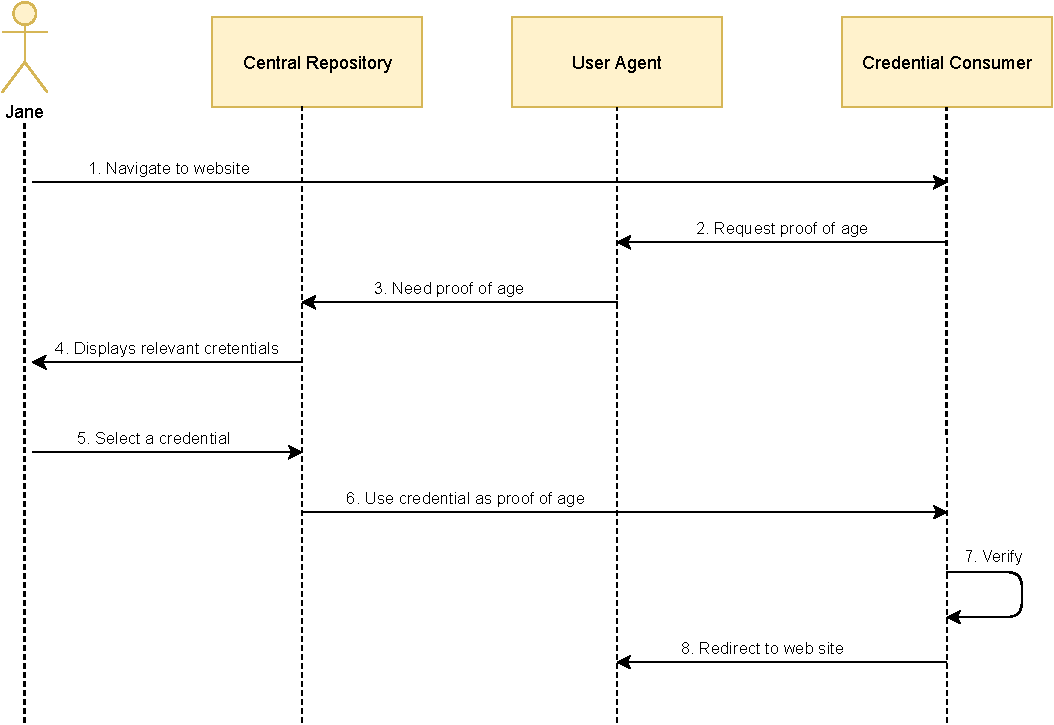
\includegraphics[width=\textwidth]{assets/informationFlow.pdf}
    \caption{An example of age verification flow from \cite{eidas}}
    \label{fig:Verification flow}
\end{figure}





\section{Suitable process for digitization}

We have discussed a huge potential of blockchain and smart contract use in eCommerce, and we have introduced a few real projects. One of the core processes and the most critical part is payment. With a payment process, yet another responsibility, like a buyer's protection and refunds appear. When the payment process is well designed, another discussed improvements and effects of using smart contracts as fraud reduction and genuine reviews appear almost naturally. Therefore, our scope of interest for the rest of this thesis is the process of online order that focuses on payment and buyer protection.



\chapter{Analyses of an online store order process}

% Talking, what will be in this chapter
This chapter introduces the process of an online store order with a description of each process's mandatory aspects.  It starts with a detailed analysis of the as-is model. We will look at the order as a state machine and talk about possible cases in each state. The review of the existing solutions and buyer protection are critical topics to truly understand the business idea of the whole to-be model.

The to-be model is designed based on provided functional and non-functional requirements. Included use cases fulfil each functional requirement. 

The last section, technological architecture, contains a technical and architectural solution for the introduced to-be model. It discusses the data model and the composition of the smart contracts with an idea of future technological solution design.


\section{Process of an online store order} 

This observation is focused on Slovak e-commerce market, but a proper explanation is provided for every mentioned element. In other European countries, the principles are similar, and you can easily find the described patterns all-around word. We also mention a few world-wide examples.

Before the start of this process, customer checks if the store has their product. If not, there is no reason to continue. This model also does not cover all details, as for example, the customer commonly looks up more online stores with interested products, and then they decide themselves based on their personal preferences. 

In most cases, when choosing the right store, the important factors are: the price of the products, the credibility of the store, the price for delivery, payment methods, the design of the store, its marketing and so on. There is a lot of subjective factors. The process is focused closely on the ordering part and events after the order is placed.


\begin{figure}[ht!]
    \centering
    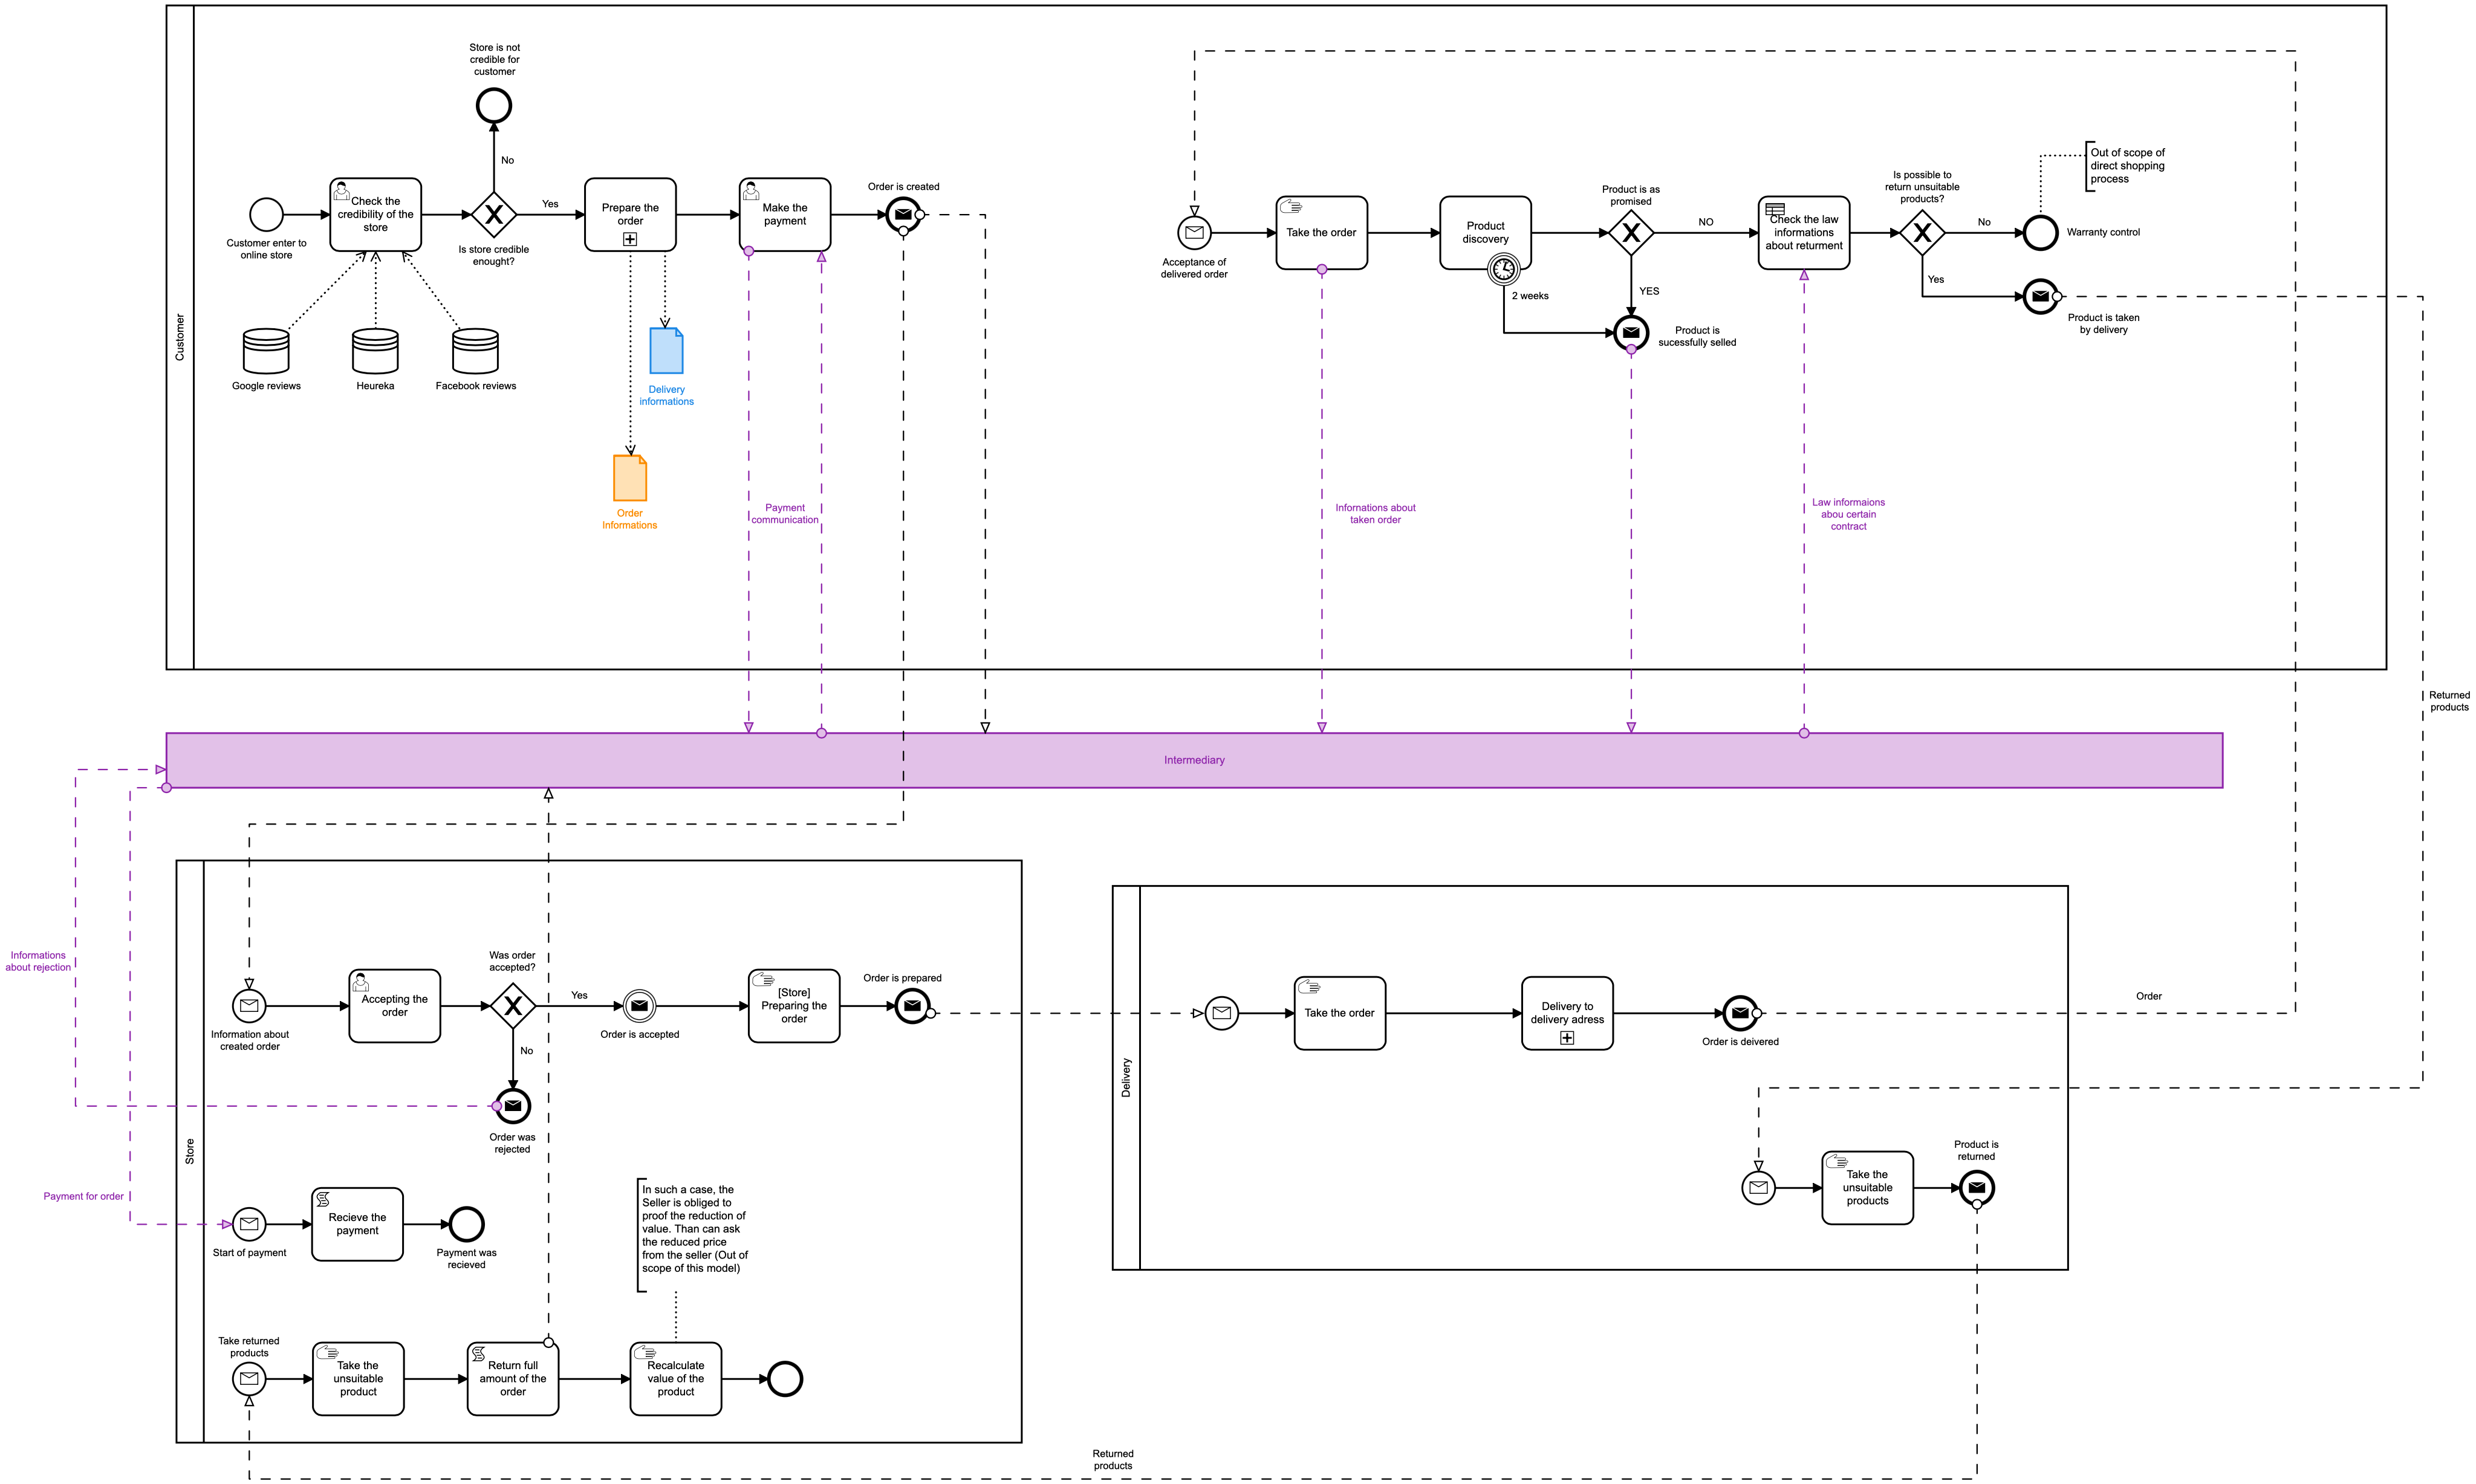
\includegraphics[width=\textwidth]{assets/As-is model.png}
    \caption{Overview of as-is model of online order (full size: EA1)}
    \label{fig:AsIsOrderModel}
\end{figure}





\begin{description} \label{reviews}
\item[Check the credibility of the store:]
One of the first things the customer is interested in is if the chosen store is credible and can fulfil the customer's needs (not only from the product point of view but also from the service perspective). The most frequent ways, how to find the credibility of online stores in Slovakia are:
\begin{description}

\item[Google reviews: ] To have Google reviews, it is necessary to have Google business account \cite{googleBusiness}, where the creator has to have basic verification. Google account users can then leave a review for its business (the reviewer has to have a Google account). The reviewer can leave a review without verification of buying service (can review everything, not only products or service, so it is possible to leave a review without relevant experience). All reviewers are almost anonymous (Google knows basic information about tel. number, which cannot be taken as identifying information). We can judge reviewer credibility based on the numbers of reviews and the local guide mark. 

Stores can defend themselves against bad reviews by comment replays with an explanation. It is also not easy to fight against fake reviews and businesses have to solve every comment individually. \cite{googleReviews}

\item[Heureka: ] Heureka started as a product price comparator and nowadays is also used to review products and online stores. Being on the marker for years, it is a trusted website and is used by smaller and medium e-shops. What is interested is that Heureka is providing a mark "verified by customers" to guarantee e-shop reliability. This mark is given to an e-shop when it completes defined conditions. 
When a store is a partner of Heureka and a customer makes a purchase, after 10 days, Heuraka sends an email with a custom link bound to their order. With this link the customer is redirected to a web form, where they leave a review (if they recommend/not recommend the store, questions about the store and product quality etc.) This guarantees that the review is based on a real order. The store with enough recommendation reviews can have the credibility mark (90\% of satisfied customers and tens of reviews or 97\% of satisfied customers and hundreds based on mark colour).
In this case, a reviewer is anonymous for a reader of the reviews (store can link order with a review), but the review is based on the actual order. The store can defend itself by responding to the review. \cite{overenozakazniky}

\item[Facebook reviews:]
For this kind of reviews, store has to have a Facebook page. Then every Facebook user can leave a review on the store's Facebook site. These reviews are not linked to orders. It means that every user can leave their opinion similarly to google reviews. The difference is that users are not (mostly) anonymous (this is questionable, but by the Facebook policy, we will assume this state). It is possible to have a fake account, but it is straightforward to fight against reviews from these kinds of accounts. Also not every store has these reviews public; there is an option to hide reviews. Stores can defend themselves as in previous examples by commenting the review. \cite{facebookReviews}

% Zlavomat


\end{description}

These representatives were chosen based on the digital report of Slovakia in 2020 \cite{dataportal}, where Google is the most visited site in Slovakia. Facebook is 5-th most visited site and the most popular social network (based on total active users). Heureka is the most visited e-commerce site in Slovakia (\cite{similarHeureka} and \cite{heurekaPropag}). This method is also recommended by the network of European Consumer Centers ECC-Net \cite{ecc}.

If there are not enough reviews in these places and the customers are still willing to buy, they pay significantly more attention to the payment methods with buyers' protection.


\item[Preparing the order:]
This step is individual for every store. The main goals are placing items into the basket, entering the discount code/coupon, and providing the mandatory information to complete the order, such as the payer information and delivery information. In this step, there can be some store-specific forms, for example, the delivery date or notes for the store. Commonly customer can choose the delivery company and payment method, which we discuss in the next step.

\item[Making the payment:]
The exact execution of this action depends on the chosen payment method discussed in \ref{paymentmethods}. This model counts on a payment method which goes through an intermediary (Paypal, Klarna and so on). The customer sends the payment to the intermediary bank account, and it informs the store about a successful payment. When the customer is registered in the intermediary system, it usually only accepts the payment. If they doesn't have an account, they will need to enter credit card information. They also see the order details, which the intermediary will save to its database. This re-saving prevents the store from changing the information on its side.


\item[Accepting the order:]
As discussed before in the purchase contract \ref{purchaseContract}, the seller can also withdraw from the contract.

\item[Preparing the order:]
This is an individual process for every online store. Some have their own stocks, others use external supplies or a drop-shipping. 
In this step the store can customize the product or produce the whole product, when it is custom made. The model is not covering this process deeper, because of the individuality. The important thing is that the result of this activity is a shipment-ready product.

\item[Delivery:]
We have discussed and described the delivery methods in \ref{deliveryMethods}. This model represents the courier delivery method with authentication. It is not a necessary confirmation mechanism.
Suppose the box or the package is damaged. Is it possible with a delivery guy to write a report about the delivery condition, which can be used as evidence in the case of a dispute later. 

\item[Product discovery:]

The 14 days period after receiving goods is called a product discovery in this model . A few things can happen in this action. We will go through them in chronological order.
After opening the package, the received goods are:
\begin{description}

\item[Not the ordered one:] The product is significantly different from the described one (has another colour, size, ...) or doesn't have supposed functionality, the customer can withdraw from the purchase contract. 
%(What if is not returnable?)

\item[Goods are defective:] This case will be not covered in this model because the next step is a claim for goods, and the claim is out of our scope of interest. If the goods are damaged, the customer can't simply return the goods because the store can ask for a price difference. 
In the as-is model, the customer has to contact the seller and start the claim process. If there is a problem with communication, the customer can open a dispute via the intermediary and provide them an evidence of damaged goods. 
\end{description}

If the products are without a problem customer has 14 days to explore their functionality and in case that the customer is not satisfied, they can withdraw from the contract and return all of the ordered products. A lot of stores (mainly with clothes) offer to return only a part of the order. In this situation, we are not talking about withdrawing from the contract. Some stores even offer pay return postage. This model works with the possibility to return only part of the order. The difference is discussed later in \ref{orderAsStateMachine}.

If the customer is satisfied with the products after 14 days, the order is considered successfully completed. Any other problems are solved by the claim process based on its warranty.

The exceptions from this return possibility are mentioned in \ref{purchaseContract}. If any problem occurs with these kinds of products the solution is the claim process. 

\item[Product return:]
The customer must send the unwanted products back to the store no later than 14 days after notifying the store about the withdrawal from the purchase contract. Shipping costs are paid by the customer, unless otherwise stated in the terms and conditions.
The store can also provide the possibility of self-removal or delivery of products at the store's preferred location.

After receiving the products, the store checks the condition of the products. The shop is obliged to return the full amount paid to the seller, including the cheapest postage offered unless otherwise stated in the contractual conditions.

If the product's condition is undesirable (the goods have been handled beyond normal handling), the store may claim damages from the customer for restoration to the normal state. However, the amount requested may not exceed the value of the product.\cite{customerProtection} The reduction of the product price is obligatory to prove by the store.

\end{description}


\section{Order as a state machine} \label{orderAsStateMachine}

It is suitable to think about an order as a state machine. It can be divided into non-looping stages which rapidly helps to lower complexity in describing requirements and decide what is possible to do in every step. See figure \ref{fig:orderStateMachine} where the states are visualised. These stages will be used later in \ref{functionalRequirements}. We assume an intermediary for payment in these stages. Follows the description of the states:

\begin{figure}[ht!]
    \centering
    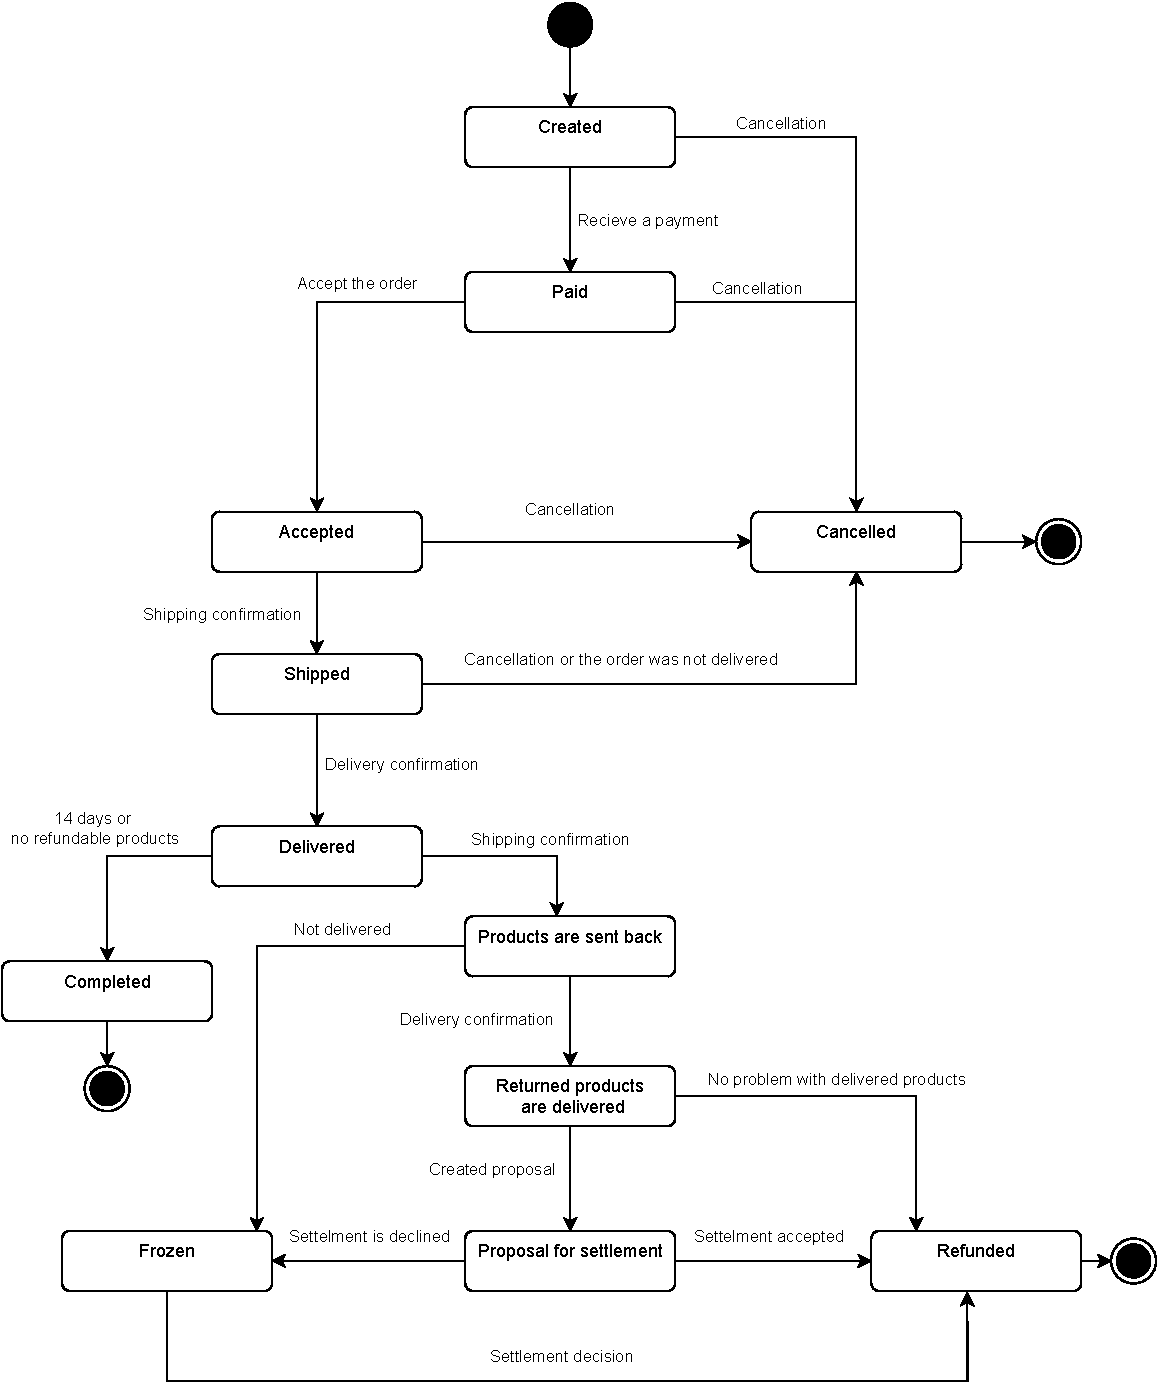
\includegraphics[width=\textwidth]{assets/OrderStateMachine2.pdf}
    \caption{Order as a state machine}
    \label{fig:orderStateMachine}
\end{figure}


\begin{description}

\item[Created:]
It is the initial state of the order. It defines the ordered products, its method and price.

\item[Paid:]
This state occurs when the customer pays for the order. The payment doesn't have to be necessarily at the store's account.

\item[Cancelled:]
As described before in \ref{purchaseContract}, the store can cancel the order for various reasons. 
Also, if the store is unable to accept the order (take a long time), the customer can cancel the order.

\item[Accepted:]
This state becomes after accepting the order. When the order is transferred to this state, it also starts encountering time to delivery. The store has limited time for the delivery (from law \cite{customerProtection} it is 30 days, but the store can change this delivery time in their terms and conditions document). 

\item[Delivered:]
The order is in this state when the customer receives the goods.
If the order has a returnable product, it will be in this state for 14 days and then will transfer to a Completed state, or the customer will want to return it.
If there are no returnable products, the order is automatically transferred to the Completed state.

\item[Completed:]
The order is completed and the store can receive the money for the order. This is the end-state for the order. The purchase process can continue by starting an warranty case, but this is out of the order process scope. 

\item[Products are sent back:]
Suppose the customer decides to return some (or all) returnable products. This state also depends on the Terms and conditions of every store individually. 
By the law discussed before in \ref{purchaseContract}, the customer has to return all products, but some stores (especially with clothes) give customers the ability to return only a part of the order. The customer has to return every gift provided with the goods (if it is linked to returning goods.)

\item[Returned products are delivered:]
The store confirms delivered product and checks the condition of the goods. If everything is right, the next state is the refund.  If not, the store can ask for compensation for damaged goods, and the order continues to Proposal for settlement.

\item[Proposal for settlement:]
The customer can agree with the Proposal and then the order continues to the refund state or they can disagree and then open a dispute and the order continues to Frozen state. 

\item[Frozen:]
The intermediary will decide which side is right and settle the refund.

\item[Refund:]
The proper amount of price will be sent to both accounts. Here are three cases, based on which way did the order came to this stage.
\begin{itemize}

\item From \texttt{Returned products are delivered}, that means that all the goods were returned, and the full price of the returned products will be sent to the customer account.
\item From \texttt{Proposal for settlement} means that the customer agreed to the reduced return price, and the agreed amount will be sent to their account. The difference between the paid and returned price is sent to the store account.
\item From \texttt{Frozen} state, it depends on the decision of the intermediary. The decided amount will be sent to both the accounts.
\end{itemize}
In case of returning all the goods, the price for the cheapest offered delivery solution is returned to the customer account (if it is not defined in ToC  to return full delivery price).
\end{description}




\label{existingSolutions}
\section{Existing solutions on the market}

% Paypal
% Klarna

This section describes the working principle of intermediaries as a payment solution for online stores. It informs about benefits for buyer and seller and about fees for providing this type of services. Pieces of information are taken from Paypay official website and Klarna official website and merged in order to offer non-domain specific description. We follow up on the information provided in \ref{paymentmethods}.

The intermediary solutions are provided by highly trusted companies. They are offering buyers protection service, which the buyer can use when any problem with a transaction made through them occurs. The customer can register an account in these companies and save their credit card information. They can see the whole transaction history in their account with an option to open a dispute about a concrete transaction. The intermediaries are also providing advantages as a mobile application for easier use.

From a business point of view, it is advantageous to use an intermediary for several reasons. When it comes to a new store, offering a payment with the buyer's protection increases the credibility of the store and the customer feels covered in case of a problem.

Another significant advantage is that the intermediary stores the information about payment cards, so it is their responsibility to protect them. The intermediary also provides a payment gateway and a payment mechanism, which is advantageous, especially for new e-shops. Most pre-programmed e-shop systems offer a built-in integration of these payment solutions, or the payment intermediary also often provides a plug-in for these systems.

On the other hand, the intermediary wants a fee for each mediated payment, which consists of a fixed amount per transaction and a variable percentage of the amount of the transaction. The store may also be charged fees for resolving customers' opened dispute (dispute fee / high volume dispute fee). As mentioned above, the transaction's money does not go directly to the store account but to the intermediary account and to the store account, still in their own system. These funds (after deducting fees) can be withdrawn by the store, which in some instances may also be for a fee.

% Image of working paypal


\subsection{Buyers protection}

This service's main idea is to protect the consumer from ending up without the purchased goods and the money they paid for it. Before we go to further, we need to define the following terms, according to the definition of PayPal:
\begin{description}
\item[Proof of shipment]
- Online or physical document from the delivery company, where you can see the date of shipment together with the customer's address entered when ordering. This address must include at least a city, country, or ZIP / Postal code or equivalent.

\item[Proof of delivery]
- Online or physical document from the delivery company, where you can see the date of shipment, the customer's address entered when ordering. This address must include at least a city, country, or ZIP / Postal code or equivalent.
Signature confirmation is an online document on the company's website, indicating that it was signed. In other words, the shipping company can prove the deliver status.
\end{description}

Consumers can use this program in two cases, namely
\begin{description}

\item[When products never arrived:]
In this case, proof of shipment or proof of delivery based on the value of the goods will be required from the trader.


\item[When the item significantly differs form its description:]
We have described a few cases in \ref{orderAsStateMachine}, so now examples from PayPal website tell more than definitions
\begin{itemize}
\item You received a completely different item. 
\item Example: You purchased a book, but received a DVD.
\item The item is missing parts or features, and this was not disclosed. 
\item Example: The listing said batteries included, but they weren't.
\item You purchased a specific quantity of an item, but received the wrong amount. 
\item Example: You purchased five pairs of fuzzy dice and only received four.
\item The item was damaged en route to its destination. 
\item Example: You bought a beautiful antique lamp, and it arrived in pieces.
\item You received a counterfeit version of the item.
\item Example: You purchased a Rolex, but received a Faux-Lex.
\end{itemize}
\end{description}


\subsection{Buyers Protection process}


\begin{description}

\item[Start a dispute:] The customer starts a dispute process by a conversation with the seller. If they are not able to reach an agreement, they involve the intermediary.

\item[Intermediary involution:] The intermediary starts paying attention to this case. It reads the conversation between the customer and the seller. 

\item [Presenting documents, information, and proofs:] When the intermediary gets acquainted with the problem's circumstances, it may ask the customer and seller for the documents and evidence that proves them right. From the customer, it can ask a photo or video of received goods or the record of receiving protocol if the package had noticeable damages. From the seller, it can ask a proof of shipment or a proof of delivery. 

\item[Shipping request:] By moderating the situation by the intermediary, it can ask the customer to send the goods back to the seller, to the intermediary or to a third party and provide a proof of shipment or a proof of delivery. 

\item [Final decision:] After considering all facts, evidence and documents, the intermediary decides the occurred situation's solution.
\end{description}

\label{tobeModel}
\section{To be model}
This section provides a description of the to-be model. The purpose of to-be model is to replace the intermediary for payment in the as-is model. Have a closer look at figure \ref{fig:ToBeOrderModel}, where the to-be model is modelled in BPMN. The goal was to change the original as-is model \ref{fig:AsIsOrderModel} as little as possible, ideally only to replace third-party intermediary to the smart contract. Of course, it is not that easy, but the presented model is significantly close to the as-is model to provide the most similar experience for the user. 

Orange colour marks the state changes of the order described in section \ref{orderAsStateMachine}. The model also doesn't provide all details as all possible cancellations because its purpose is to describe basic behaviour.

It is possible to observe a few differences. For example, the model doesn't end by taking the goods by the customer and providing a kind of seller protection in the form of a proposal for settlement. 

% BPMN to be model 
% description of this model
% goal was to change the process as little as possible
% 


\begin{figure}[ht!]
    \centering
    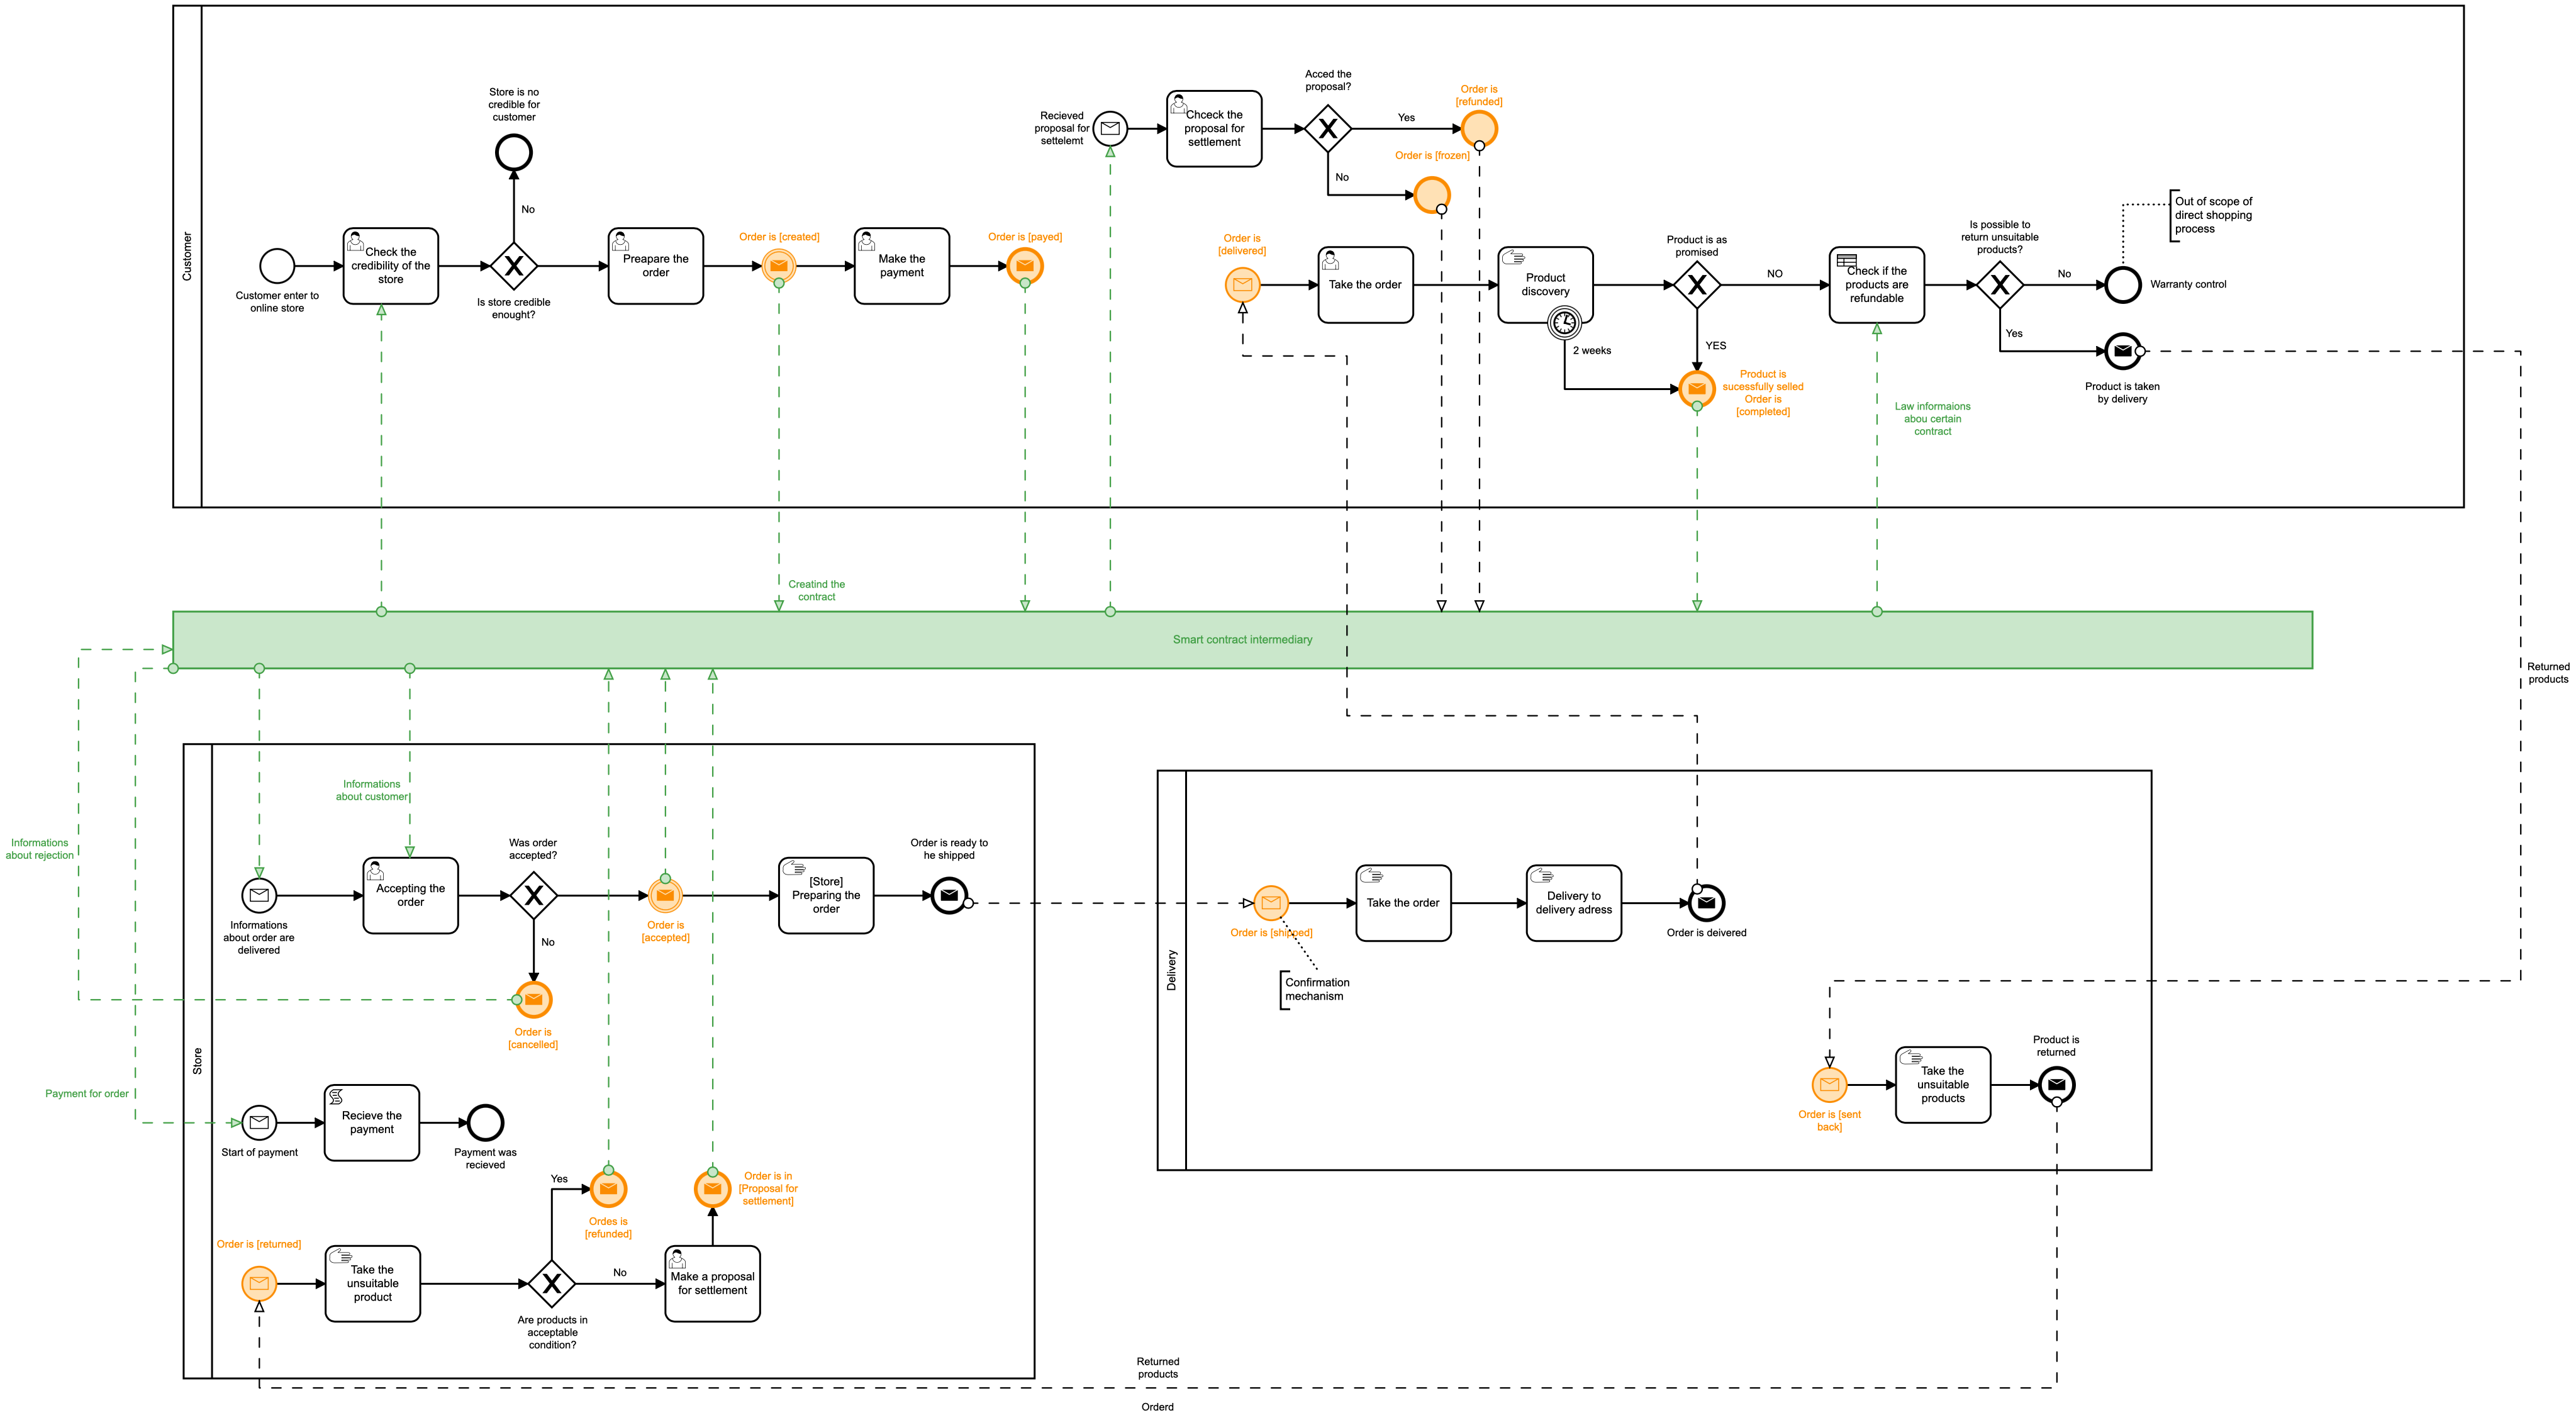
\includegraphics[width=\textwidth]{assets/to-beProcessModel.png}
    \caption{Overview of to-be order model  (full size: EA2)}
    \label{fig:ToBeOrderModel}
\end{figure}

\label{functionalRequirements}
\subsection{Functional requirements}

Functional requirements are used to express and define the behavioural and business functionality of the system. In table \ref{functional requirements} are provided functional requirements for the to-be system.

The first three requirements are also discoverable in the as-is model so that the system's idea does not change. The F4 is essential functionality for the frozen state of the order and for the system's legal site. The last requirement F5 is for supporting advantages for the public and the ability to use the full immutable and public power of the blockchain technology.
The functional requirements are later fulfilled by use cases.

% Business needs - for why we have this requirements
% Requirements are fulfilled by use cases
% with a link to the table
%




\begin{table}[ht! ]
\caption{Functional requirements} \label{functional requirements}
\begin{tabular}{| p{0.5cm} | p{2.5cm} | p{9cm} | }
\toprule
FR &
  Name &
  Description \\ \midrule
F1 &
  Order\break management &
  The system provides functionality for order management, such as creating an order, manipulation with an order based on the order's stare, and cancelling the order. The system can't delete an order. \\\hline
F2 &
  Shipping\break confirmation &
  The system has functionality for confirming the delivery state only. The system doesn't have functionality for advanced delivery management, such as claim management or delivery tracking. The system optionally supports third party integration, where it is possible to provide additional information (link for third party website).  \\\hline
F3 &
  Buyers\break protection &
  The system has buyers protection policy. That means, the payments cannot be withdrawn from the system before both sites accept the completeness of commitments. Otherwise the system escalates and holds the payment while the authority makes a decision.  \\\hline
F4 &
  Intervention of authority &
  The system can be intervened by an authority (government, legal judgment, ministry), but only in a special frozen state. An authorized entity can intermediate the frozen state. The authorized entity is specified in the system. \\\hline
F5 &
  Providing information &
  The system provides public information about orders but covers personal data. Anyone can see all orders from the store and orders from a specific customer. But customers have to be anonimized (no personal information revealed to unauthorized entities).  \\\hline
\end{tabular}
\end{table}



\subsection{Non-functional requirements}

The non-functional requirements are system restrictions. Table \ref{nonFunctional requirements} is an overview of the non-functional requirements required from to-be system. These requirements capture the system from different perspectives as accessibility, availability, deployment, documentation, maintainability, licence, regulations, privacy, compatibility, usability, device supportiveness, security, cost elements and more. 


% Look at SI a write any defintion
% with a link to the table
%


\begin{table}[ht!]
\caption{Owerview of non-functional requirements} \label{nonFunctional requirements}
\begin{tabular}{| p{0.5cm} | p{2.5cm} | p{10cm}|}
\toprule
NR &
  Name &
  Descruption \\ \midrule
N1 &
  Public acces &
  The system is publicly accessible, with the requirement that the user has to have a supported browser or application to interact with javascript and crypto wallet (Metamask). \\ \hline
N2 &
  Public availability &
  The system has no granted accessibility. Accessibility is based on access to Ethereum network and acces providers. System is independent from falling the acces provider (store hosting). Universal acces point is not included. \\ \hline
N3 &
  Deployment to online store solution, Store aviability &
  The system can be provided as a plug-in into online store solutions. The pre-programmed solution is not included. The online stores have to provide defined API by the system. The deployed environment has to support JavaScript and has a connection to the Ethereum network. \\ \hline
N4 &
  Documentation of the smart contract &
  Smart contract has a public documentation which describes the interaction with it. \\ \hline
N5 &
  Maintainability of application &
  The application software is possible to maintain by plug-in updates. \\ \hline
N6 &
  Maintainability of smart contract &
  The smart contract is not possible to update. Smart contract requires to deploy a new one in case of law changes. \\ \hline
N7 &
  Open-source &
  The software is provided as open-source. \\ \hline
N8 &
  Law regulations &
  System support law codex of the specified country but only to the date of last change... \\ \hline
N9 &
  Privacy policy &
  The system respects the protection of personal data with the exception of the right to be forgotten. The orders are not possible to delete, but the customer is anonym from the public site of view... \\ \hline
N10 &
  Platform compatibility &
  System is compatible with all platforms supporting acces requirements. \\ \hline
N11 &
  Usability &
  The system has a similar behaviour as classical payment methods thought intermediary. In every state, the user knows the possible next steps. \\ \hline
N12 &
  Device support &
  The system is supported on all devices supported access requirements N1. \\ \hline
N13 &
  Identification &
  The user is identified by his account ID and password is his private key for signing the transactions. \\ \hline
N14 &
  Cost &
  Users (customers, online stores, and deliver) is paying a transaction fee for every change of order's state. Providing information is free.  \\ \hline
\end{tabular}
\end{table}


\subsection{Use cases}

% For what use cases are
% provide the 2.x description
% for better understanding are use cases supported by wire frames
%

Use cases describe system interactions with external entities (as actors) and the accessibility of the pieces of information for concreate user roles. Use cases for the system are provided by marking Y.X, where Y is describing the group similarity and X the concrete case. Each use case has a mark, name, description, optionally pre-conditions and post-conditions, extension (is extended by) and the authorised roles.
All use cases are provided as the attachment EA3 to this thesis, so now we describes only a few representatives from chosen categories. The description provided here is only to understand the idea of the case. Before embarking on the presentation of use cases, focus your attention on the figure \ref{fig:actors} that illustrates the system's role. The public, customer, store, deliverer are pretty self-describing and the authority role comes from F5 (functional requirement 5 in table \ref{functional requirements}) and N8 (non-functional requirement in table \ref{nonFunctional requirements}).
\begin{itemize}
\item The first UC1 implements \ref{useCase1} the basic requirement for interacting with a system, and it is available for a public role.

\item Group 2.X are information providers. Their purpose is to select information that is available to certain roles in given situations. They are mostly used as an extension for other use cases. They primary contain exact attributes, which are used later in the data model. Chosen representatives are in table \ref{useCase2.4} and \ref{useCase2.6}.

\item Group 3.X contains the use cases which represent the interactions which are changing the order state. The state changes are observable in pre and post conditions. They realize the intercommunication between parties and implement the logic of the order process. The representatives of this category are in tables \ref{useCase3.2} and \ref{useCase3.6}.

\item Group 4.X carries the public interaction with the system. Together with group 5, it offers the views to the lists of orders. The representative is \ref{useCase4.1}

\item Groups 6, 7 and 8 include the functionality for system management and maintainability. The representative is \ref{useCase6}

\end{itemize}





\begin{figure}[ht!]
    \centering
    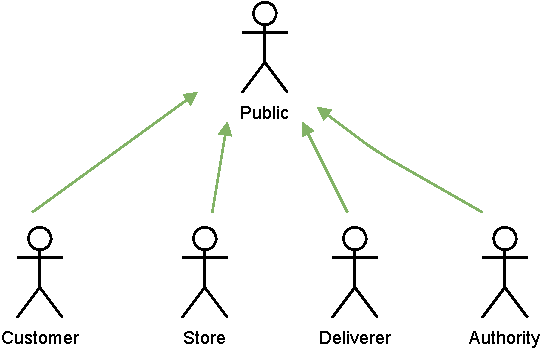
\includegraphics[width=0.5\textwidth]{assets/Actors.pdf}
    \caption{Order actors}
    \label{fig:actors}
\end{figure}


\begin{table}[ht!]
\caption{Use case 1} \label{useCase1}
\begin{tabular}{| p{3cm} | p{10cm}|}
\hline
Use case & UC1    \\\hline
Name     & Log in \\\hline
Description    & The user can log in to the system through his crypto wallet (Metamask). \\\hline
Pre-conditions & Ethereum account, Crypto wallet with sign in functionality              \\\hline
Roles    & Public \\\hline
\end{tabular}
\end{table}

\begin{table}[ht!]
\caption{Use case 2.4} \label{useCase2.4}
\begin{tabular}{| p{3cm} | p{10cm}|}
\hline
Use case & UC2.4    \\\hline
Name     & Deliverer details \\\hline
Description    & Deliverer details are the company account address, deliverer, who took goods from the shop and deliver, who gave goods to a customer. Optionally, when returning goods company account address, deliverer took goods from the customer and deliverer, who gave goods to a store.  \\\hline
Roles    & Customer, Store, Deliverer \\\hline
\end{tabular}
\end{table}

\begin{table}[ht!]
\caption{Use case 2.6} \label{useCase2.6}
\begin{tabular}{| p{3cm} | p{10cm}|}
\hline
Use case & UC2.6    \\\hline
Name     & Payment details \\\hline
Description    & Payment details  are cost of goods, delivery cost, tax rate, tax price in total, payment in total ( goods + delivery including tax ), additional costs ( gas fee ).  \\\hline
Roles    & Customer, Store \\\hline
\end{tabular}
\end{table}

\begin{table}[ht!]
\caption{Use case 3.2} \label{useCase3.2}
\begin{tabular}{| p{3cm} | p{10cm}|}
\hline
Use case & UC3.2    \\\hline
Name     & Pay for order \\\hline
Description    & Customer pay for the order payment in total cost plus gas fee consumed by the transaction. This gas fee is added additional cost attribute in order.  \\\hline
Pre-conditions    & OrderStare = Created \\\hline
Post-conditions    & OrderStare = Paid \\\hline
Is extended by    & UC1, UC2.X \\\hline
Roles    & Customer \\\hline
\end{tabular}
\end{table}

\begin{table}[ht!]
\caption{Use case 3.6} \label{useCase3.6}
\begin{tabular}{| p{3cm} | p{10cm}|}
\hline
Use case & UC3.6    \\\hline
Name     & Confirm receivement \\\hline
Description    & The recipient confirms the given shipment. It is possible to confirm only the whole product list, not only parts.  \\\hline
Pre-conditions    & OrderStare = Accepted or OrderStare = Shipped \\\hline
Post-conditions    & OrderStare = Shipped or OrderStare = Deliveder \\\hline
Is extended by    & if role = store or role = customer UC1, UC2.X, if role = deliverer UC1, UC2.3. UC2.4, UC2.5 \\\hline
Roles    & Customer, Store, Deliverer \\\hline
\end{tabular}
\end{table}

\begin{table}[ht!]
\caption{Use case 4.1} \label{useCase4.1}
\begin{tabular}{| p{3cm} | p{10cm}|}
\hline
Use case & UC4.1    \\\hline
Name     & Public information of store orders \\\hline
Description    & It displays the list of the store's orders and the status of the order.   \\\hline
Is extended by    & UC1 \\\hline
Roles    & Public \\\hline
\end{tabular}
\end{table}

\begin{table}[ht!]
\caption{Use case 6} \label{useCase6}
\begin{tabular}{| p{3cm} | p{10cm}|}
\hline
Use case & UC6    \\\hline
Name     & Upgrade contract \\\hline
Description    & The authority can change the address of the smart contract in the network (Migrate the contract).   \\\hline
Roles    & Authority \\\hline
\end{tabular}
\end{table}

% \subsection{Screens}



\subsection{Data model}
% As we mention begore storing data in blockchain is costly
% it is data model for client app
% storing all data is not nesessery depence on technologival architecture
% Some data can by only hast to maintain integrity
% The all data need only client application
% Talk about data 
%

As we mentioned before, storing data in blockchain is extremely costly. Therefore, it is very important to correctly select the most important data to be stored in blockchain and which in off-chain. The data model \ref{fig:dataModel} shows necessary data for a correctly working order system, but not every data has to be stored in the network. The decision, which data are stored where highly depends on the technical architecture of the system. It is always better just to re-use stored data, which are already in the network, than saving new one. We discuss the saving logic later in \ref{advancedFutureArchitecture}.

As an example of saving the place, it is unnecessary to store all product details, so we can store only a hash of the products list. For the raw data will be responsible to store, but the copy of data can have a customer as well. The contract still holds the truth of purchased goods, so the customer can easily say what they bought, and it can be easily proved by the hash. If the store tries to cheat with a purchased product, the system can have a buyer advantage mechanism in a problematic situation. The system application provides storing logic.



\begin{figure}[ht!]
    \centering
    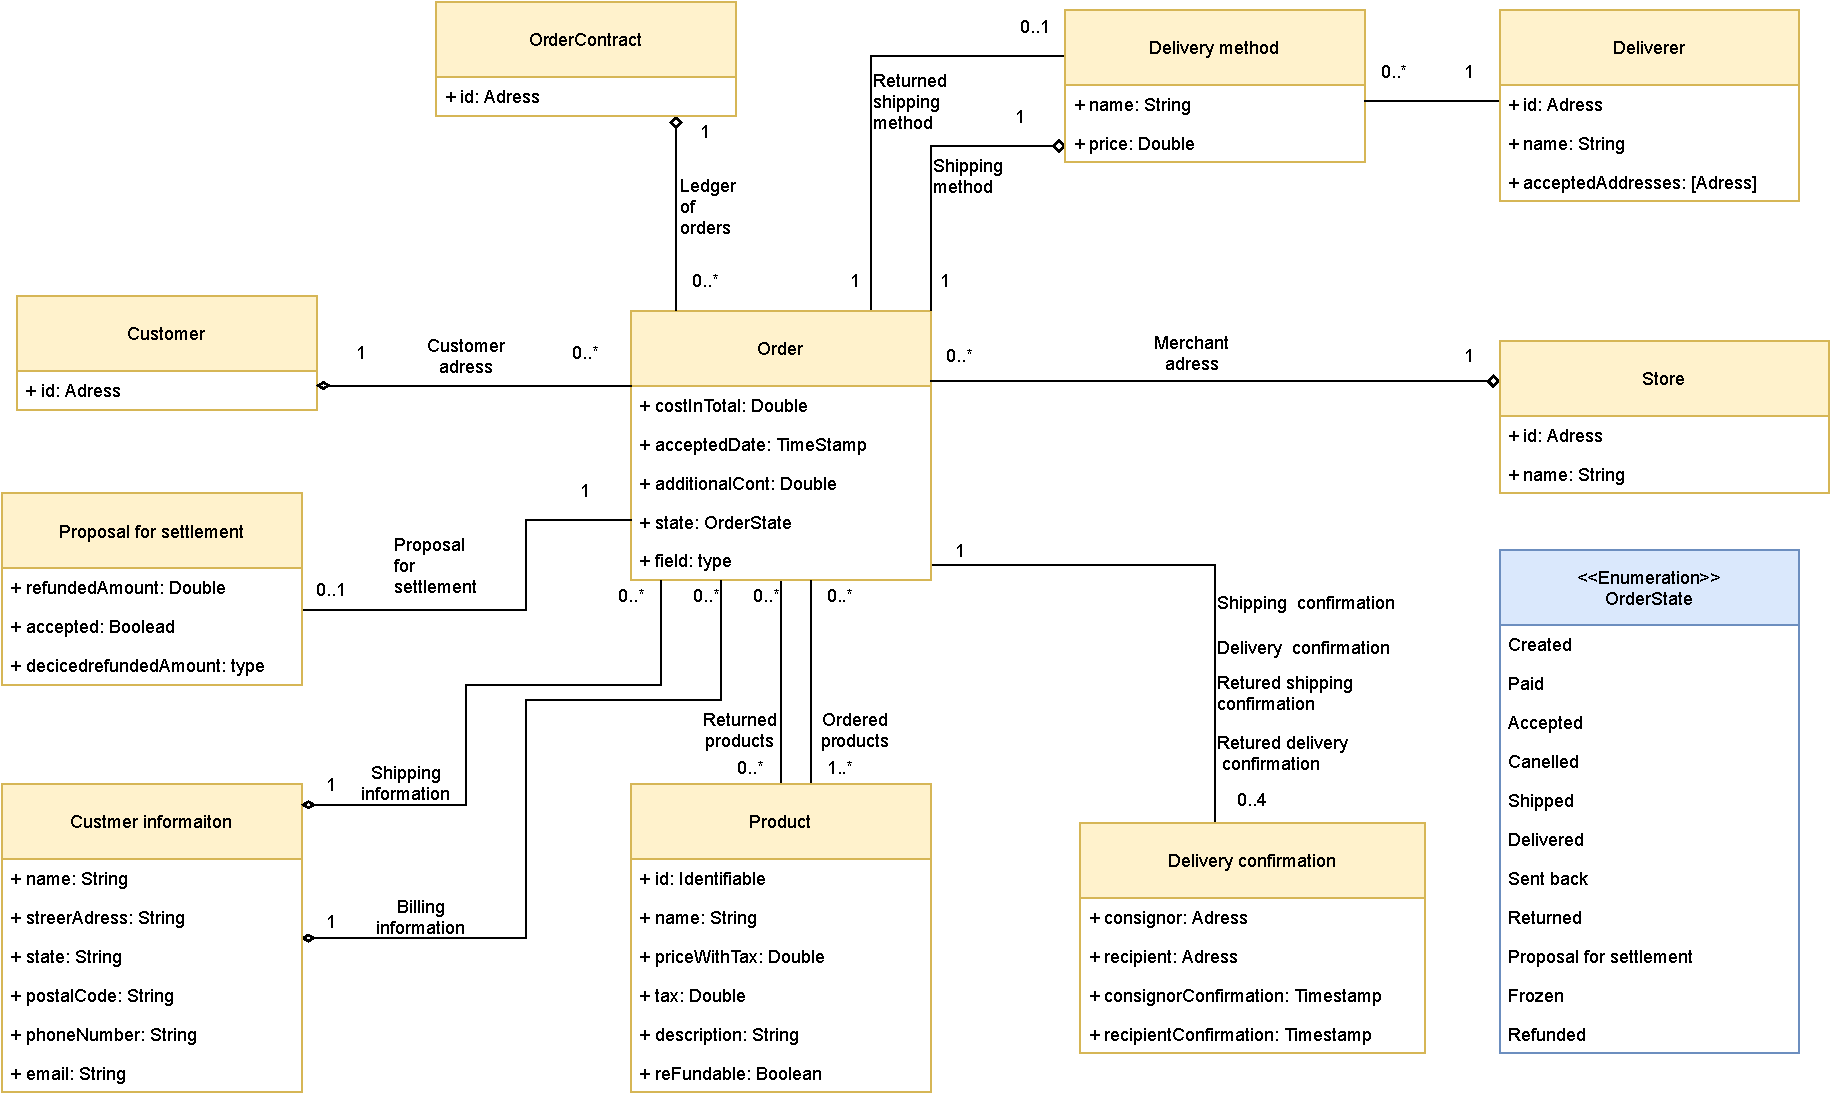
\includegraphics[width=\textwidth]{assets/DataModel.pdf}
    \caption{Das contract data model of the order process  (full size: EA9)} %Das contract data model
    \label{fig:dataModel}
\end{figure}




\section{Technological architecture}

% What we will need for creation of this system
% more solution based of usage and popularity of block chain
% weed to think about cost side of view and data distribution
% respect functional and non-functional requirements
% think about immutability of the code
% Good practises are in https://hackernoon.com/best-practices-to-level-up-your-ethereum-smart-contracts-944d5cea2cab 
% Challenge is extensibility and updates. Are a few ways ...
% 

This section contains a discussion of technological and architectural solutions of the proposed to-be system. We start with the problematic of the possibilities of dividing smart contracts within the network and take two different approaches depending on the use and popularity of blockchain. The second part of this section is a discussion of the client-side system and the possibilities of using the application as a plugin for popular online store solutions.

The proposed architecture needs to respect functional and non-functional requirements and strictly look at the cost efficiency and data distribution. It is challenging to achieving a maintainable solution, especially with the immutability of code, but it is not impossible. We use the best practices from \cite{smartContractUpgradeble} to achieve suitable architecture for specified requirements. 

You can see high-level technological architecture in figure \ref{fig:highlevelArchitecture}, and this architecture is a core for all discussed possibilities. We later specify each part of the architecture and dApp integration as a frontend. The backend part will be Ethereum blockchain and smart contracts. We use the development principle described in \cite{agiledevmethod} and some methodology ideas from \cite{workers}.

% Dapp interactin with blockchain image

\begin{figure}[ht!]
    \centering
    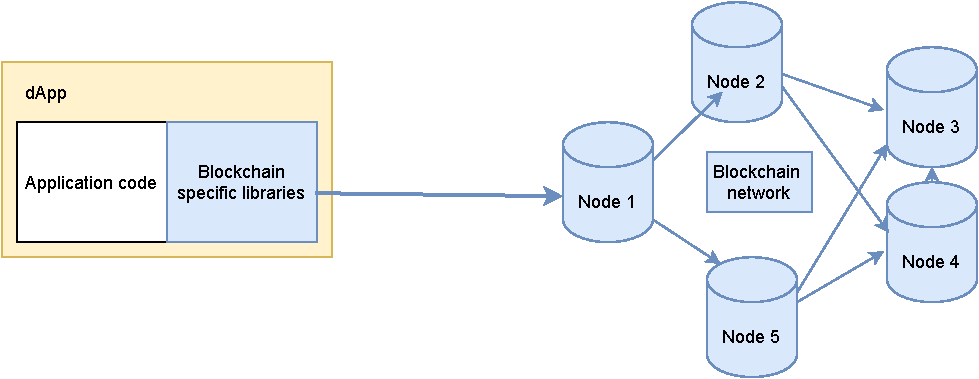
\includegraphics[width=\textwidth]{assets/highLevelArchitecture.pdf}
    \caption{High level technological architecture \cite{Singhal2018} }
    \label{fig:highlevelArchitecture}
\end{figure}



\subsection{Smart contract composition}


% Firstly we describe a smart contracts
% We have talked about characteristics in [] and we need to use qualitees.  
% cant be dependent on the contrete frontend application
% open to support third party solution
% proces is builded by DasContract metodology 
% Factors: can be deviated form Non-functional requirements
% - 
% -
% -
% -
% -
% -
% -

The first huge challenge is to find the answer to the question: "How will the smart contract architecture look like?". Many factors restrict the answer to this question. Firstly, we look at the close term scenario and the fact that our system has to manage all the model processes. Later, when the smart contract became part of the casual interaction (as internet nowadays), we can talk about a genuinely cost-efficient and trusted online purchase solution.


\begin{figure}[ht!]
    \centering
    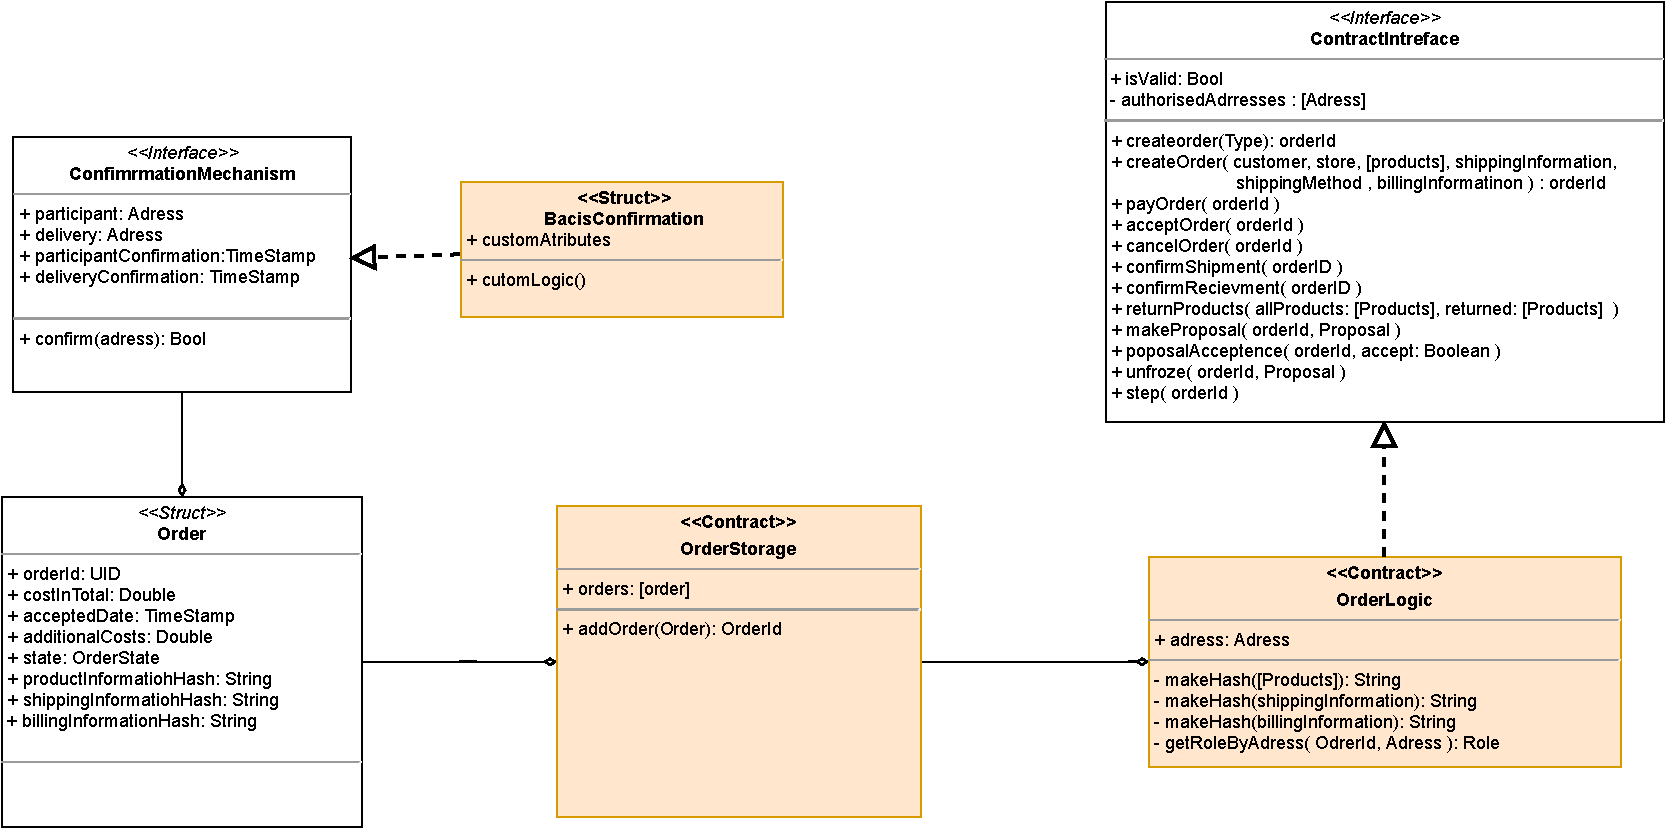
\includegraphics[width=\textwidth]{assets/SmartContractArchitecture-1_1.pdf}
    \caption{Basic smart contract architecture  (full size: EA9)}
    \label{fig:bacisSCarchitecture}
\end{figure}

\begin{figure}[ht!]
    \centering
    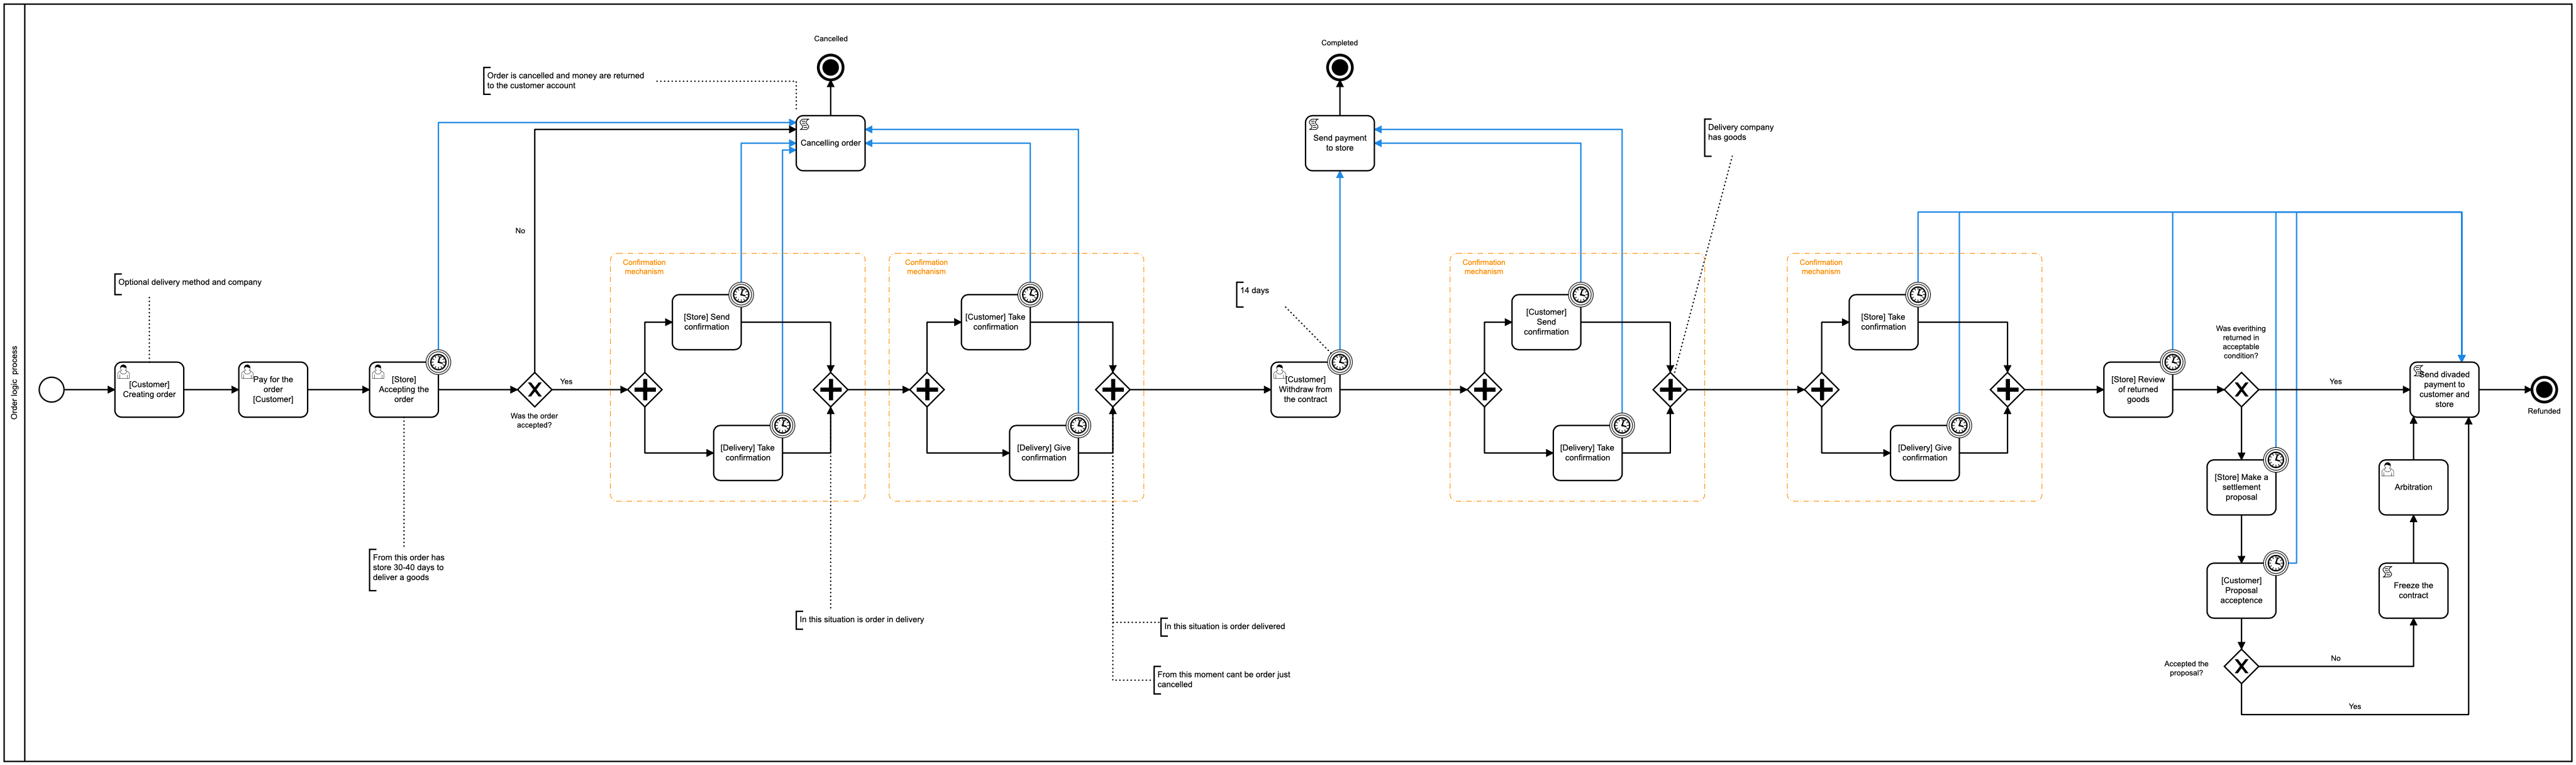
\includegraphics[width=\textwidth]{assets/smart-contract-process-diagram-with-delivery.png}
    \caption{Das Contract process model  (full size: EA4)} %Das contract data model
    \label{fig:dasContractProcess}
\end{figure}

Look at figure \ref{fig:bacisSCarchitecture}, where a UML class diagram of the first-mentioned scenario is. The smart contract composition is simple, with two contracts. The first contract \texttt{OrderLogic} represents the system's business logic and has an interface for communication with dApp. Second \texttt{OrderStorage} is a primitive smart contract, which represents the database of the orders. 

This separation has logic in the maintainability of the system. If some law changes appear or are the possibility to upgrade the business layer (we will discuss this later), we can easily change the \texttt{OrderLogic} contract with another implementation. In the real world, we can't delete the old one, but we can make internal logic to stop the interaction and, in dApps, simply change the smart contract address. The new one can easily continue where the old stopped.

To save some data storage, we have decided to store only the hashes of products, shipping information and billing information. The reason is to save the cost of storage and there is no reason to store whole data. A copy of this data can be saved by the store and (optionally) on the customer side. This solution can have a few disadvantages because in function \texttt{returnProducts( allProducts: [Products], returned: [Products] )}, the application needs to provide whole list of products. The responsibility of hash calculation is on the smart contract's side for security reasons. 

Figure \ref{fig:dasContractProcess} represents backend logic. Pay attention to the timer and flows from the timers. We can't implement exactly the same functionality because the only way to execute code in a smart contract is via transaction. No cron functions exist, so we use a step function to solve this problem, which works as a impulse to check the dated conditions and change the state. You can find a full-size process as external attachment 4 (EA4).

\label{advancedFutureArchitecture}
\subsection{Advanced future architecture}

\begin{figure}[ht!]
    \centering
    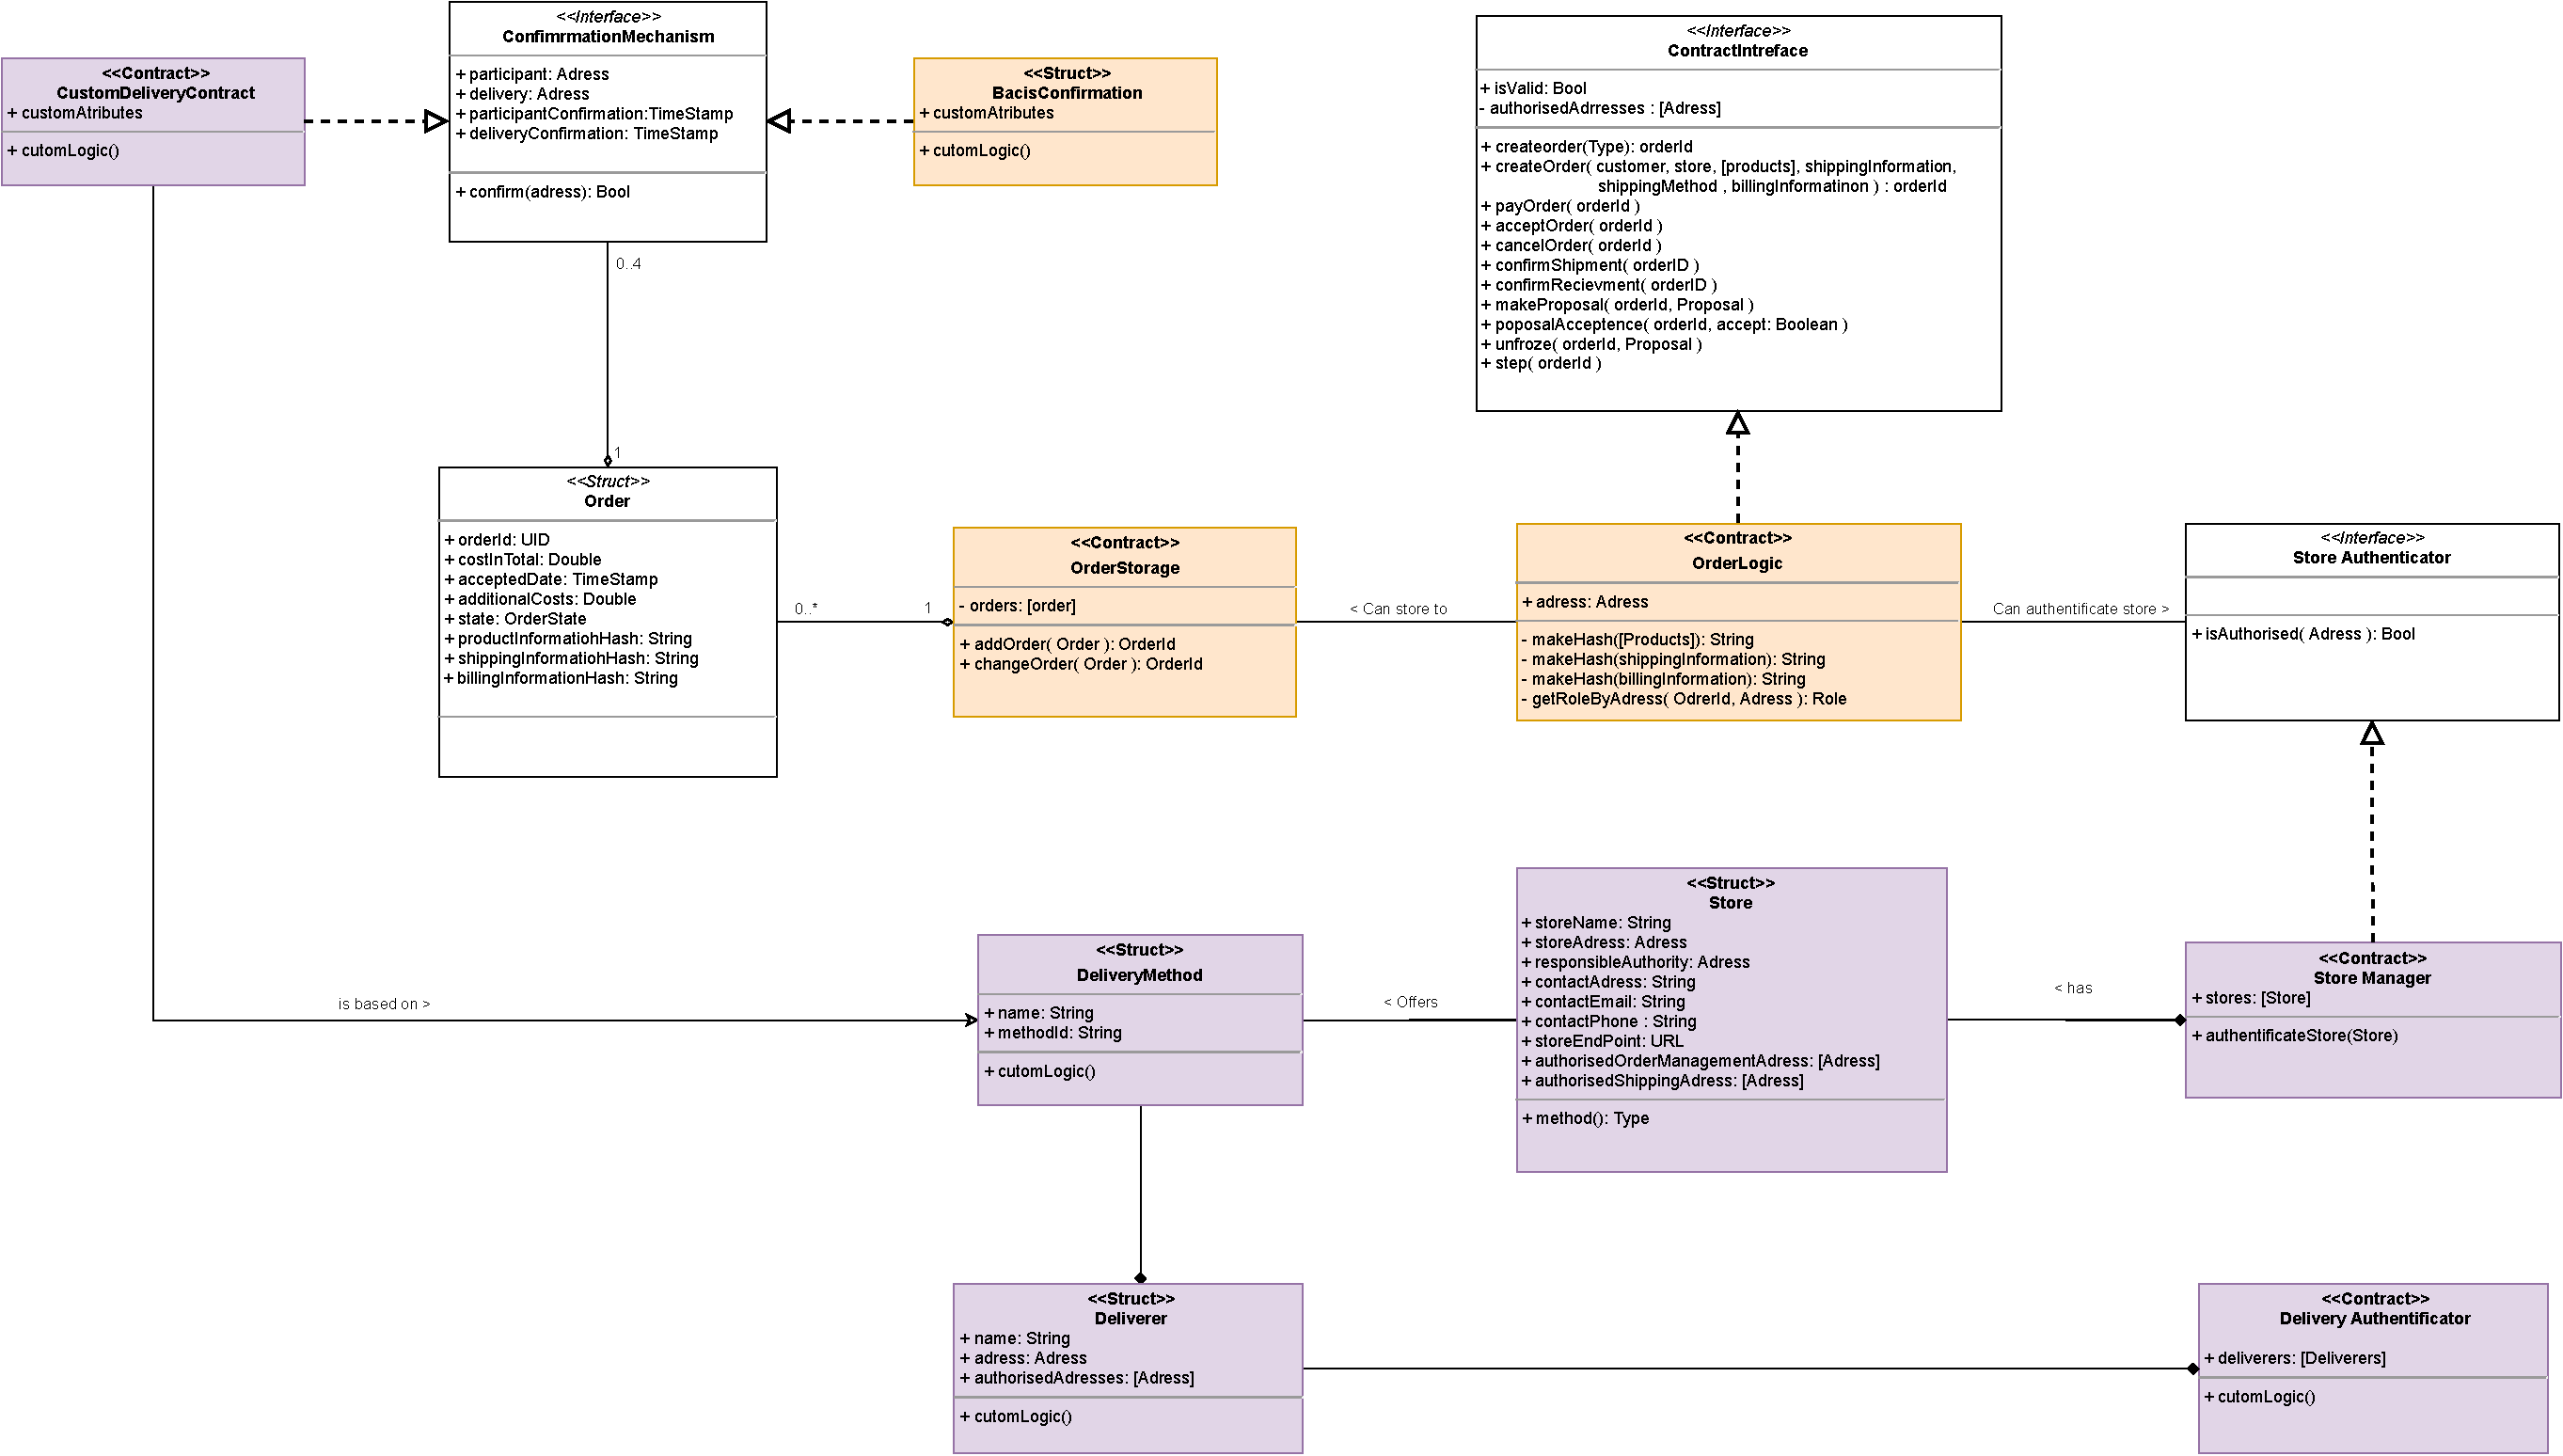
\includegraphics[width=\textwidth]{assets/SmartContractArchitecture-2_1.pdf}
    \caption{Future smart contract architecture  (full size: EA9) }
    \label{fig:futureSCarchitecture}
\end{figure}


It is not possible to predict future, but we have to design solutions that can be scaled and upgraded. When blockchain becomes more used by state authorities, our model's story can look like on figure \ref{fig:futureSCarchitecture}. The contract interface is not changed, so the interaction with dApp can be the same. 

Imagine that the store has an opportunity to register through an authority (for example a ministry) to this system. Store's information is stored in store structure, and every store is bounded to a public entity, such as a company. This system can accept only authorized stores as sellers and a buyer is no more purchasing goods from an anonymous entity. We mean anonym because the system surely now only the address of the seller. It is possible to imagine this registration as nowadays, when the store wanna accept the payments through PayPal. Firstly, it needs to register itself at PayPal as a merchant and provide some identification documents. We can apply the same pattern for delivery (or virtual identity).

The next advantage we can observe is signing the shipping confirmation or defining the internal rules for contract behaviour. Not every time the same person accepts the orders and the person who is signing the shipping contract the same. This pattern is even well suited for the delivery company. 

We mentioned that supply chain management and delivery are one of the most promising blockchain applications. In this type of process, the delivery company can have its smart contract for delivery and use it in the presented model. The only restriction is to use confirmation mechanism as an interface so that the system can work with it. 


\subsection{DApp}
% re-usable across the system
%
%
%
The dApp has to have two backend parts. The first part is the store side, where all information in the raw version is stored. This side creates a pre-defined API for dApp. The API is the same for all online store systems, so when it is delivered as a plugin to store, the programmers have to only map this functions to concreate implementation.

The second part of the backend is a blockchain side. This is the same for every implementation. DApp will interact with smart contract, which has a certain interface. Contract stores only the hashes of information stored on the store side to ensure the system's integrity. 

Utilizing this principle allows dApp to be reusable across all online store systems. For integration to the new system, it is only needed to code the store's API for dApp.


\section{Chapter summary}

We created an as-is model of online order in BPMN language with a detailed description of each part and activity. We have also produced a state diagram for order, which helps us to create specific and well-understood requirements. We have explored existing solutions on the market, highlighting the importance of the buyers' protection for business success.

Based on collected pieces of information, the to-be model was designed. We have specified the non-function and functional requirements, which were defined into the use cases. We introduced the Das Contract data model for the system entities and Das Contract process model to illustrate smart contract's behaviour.

The end of the chapter was focused on the technological architecture of the system. Two versions of the architecture were discussed with their backend and frontend parts.

% ----------------------------------PROOF OF CONCEPT------------------------------------------<<

\chapter{Proof of concept} \label{proofOfConcept}

The concept's goal is to show potential real-world implementation direction and prove the possibility of realising the described system and its ideas. It describes a working application for order management with the backend blockchain system. We will go through the introduction of used technologies, the smart contract architecture and frontend web-based application. The end of the chapter is focused on testing the implementation of smart contracts. The code snippets are provided for each part.

\section{Used technologies}

To create such a complicated system we need to choose the right technologies. Despite the fact that Ethereum is a relatively new technology, we can find exciting development tools and supporting development communities. We use Solidity language for implementing smart contract, JavaScript for testing the frontend application. The whole project is based on Node.js. Now follow our deck of tools for creating the proof of concept.

\begin{description}
    
\item[Ganache \cite{ganache}] is easy to use local Ethereum network. It provides an application or command-line interface and a fantastically quick run functionality to run local network literally with one click (or command).

\item[Truffle \cite{truffle}] framework is for developing smart contracts. We use Truffle not only for compiling and deploying created smart contract to the local network but also for testing deployed smart contracts.

\item[Chai.js \cite{chai}]is a framework for testing in javascript. It has useful functions such as asserts or shoud.be for testing smart contract response.

\item[OpenZeppeline] is as described in their website: "A library for secure smart contract development. Build on a solid foundation of community-vetted code."\cite{openeZeppelin} We use the pre-programmed library Utils to check the correctness of the smart contract address.

\item[dApp university \cite{dappUniversity}]  is a teaching programme from Gregory McCubbin, who teaches Blockchain development basics. We have used his \href{https://github.com/dappuniversity/social-network/releases/tag/28e13af}{template} as a baseline of our system. 

\item[Web3.js \cite{web3js}]is a javascript library for interacting with smart contract. It also has handy functions in web3.utils which are commonly used in the project. 

\item[Metamask \cite{metamaskWeb}] is a Chrome extension for interaction with decentralised applications and crypto wallets. It supports local hosted networks, what is mandatory for our concept. We use Metamask for signing transactions and simulating system's roles.

\item[React.js \cite{react} is a Javascript framework for building reactive frond-end application. Together with Bootstrap are an ideal combination for creating application prototypes as our proof of concept.

\end{description}



\section{Smart contract implementation}
We have created two smart contracts. The first one handles an order logic (plus order storage) and the second manages the delivery process. The order logic contract is a state-based contract (from order state described in \ref{orderAsStateMachine}), which is responsible for manipulating the order. Each order has its roles: a store, a customer and a deliverer, which are in our proof of concept user accounts, but they don't have to be. The delivery and the store can be smart contracts in the future.

Let's look at one of the smaller functions from \texttt{OrderLogicContract.sol} contract \texttt{acceptOrder(uint \_orderId) public} with all necessary aspects for understanding the contract's behaviour.

\begin{lstlisting}[caption=OrderLogicContract.sol function example]
    function acceptOrder(uint _orderId) public {
        // Make sure the id is valid
        require(_orderId > 0 && _orderId <= orderCount);
        // Fetch the post
        Order memory _order = orders[_orderId];
        // Check sender role in order
        require(_order.store == msg.sender);
        // Check state of the order
        require(_order.state == OrderState.PAID);
        // update state
        _order.state = OrderState.ACCEPTED;
        // update order
        orders[_orderId] = _order;
        // emit event
        emit OrderStateChanged( _orderId, _order.state );
    }
\end{lstlisting}

\texttt{require()} function is a perfect mechanism for not consuming an additional amount of gas for calling the function with wrong parameters or function in an unsupported stage of an order. Firstly, we check if the order exists, then if the sender of the transaction \texttt{msg.sender} is approved role for executing this function, and finally, we make sure the order is in the right state. When everything is correct, the logic is executed and the state of the order is saved. The last line is \texttt{emit} function, which is usefull for frontend applications, which can subscribe to the emitted event and then react on published events. It is a classical publisher-subscriber pattern.



\label{}
\begin{lstlisting}[caption=OrderLogicContract.sol confirmation mechanism example, label={lst:comfirmationMechanismExample}]
    function confirmationMechanism(uint _orderId, address _deliveryContractAdress ) public {
        // Check if provided address is smart contract
        require( Address.isContract(_deliveryContractAdress) );
        // Make sure the id is valid
        require(_orderId > 0 && _orderId <= orderCount);
        // Fetch the order
        Order memory _order = orders[_orderId];
        // Creating communication instance from adress
        DeliveryContract del = DeliveryContract(_deliveryContractAdress);

        if ( _order.state == OrderState.ACCEPTED ){
            // Required function of delivery contract for confirmation of
            // delivery act 
            if ( del.isConfirmed(_orderId, _order.store, _order.deliverer ) ){
                _order.state = OrderState.SHIPPED;
            }
        }else if ( _order.state == OrderState.SHIPPED ){
            ...
        // save an order    
        orders[_orderId] = _order;
        // emit event
        emit OrderStateChanged( _orderId, _order.state );
    }

\end{lstlisting}

Another interesting example of the proof of concept is listing \ref{lst:comfirmationMechanismExample}, which handles the confirmation of the delivery process. Similarly to \texttt{acceptOrder}, the function takes \texttt{orderId} parameter and address \texttt{deliveryContractAdress}. The address has to be a contract address, what we ensure with the first requirement and Address library from OpeZeppeline. It also has to be a contract implementing DeliveryConctract interface. The requirement is only to have the \texttt{isConfirmed( orderId, consignor, recipient )} function implemented for checking the confirmation of the selected tuple, based on the current state of the order. This is an example of how to open the system to enable stores and deliverers to implement their own smart contracts with custom logic.


% Communication diagram 



\section{Implementation of the frontend dApp}

The frontend application of proof of concept is like a payment gateway in today's payment solutions. It appears when the customer clicks on the pay by Ethereum button in the online store system. Then they see all the order's details and the available actions. 
The store and deliverer have a similar view as the customer, but each role sees different possible actions based on the current order's state. Notice the view of an application, with console logs for explaining what is happening in the background in figure \ref{fig:screenProofOfConcept}. There is a walk through of every screen with a state and process diagrams in external attachments EA8.

\begin{figure}[ht!]
    \centering
    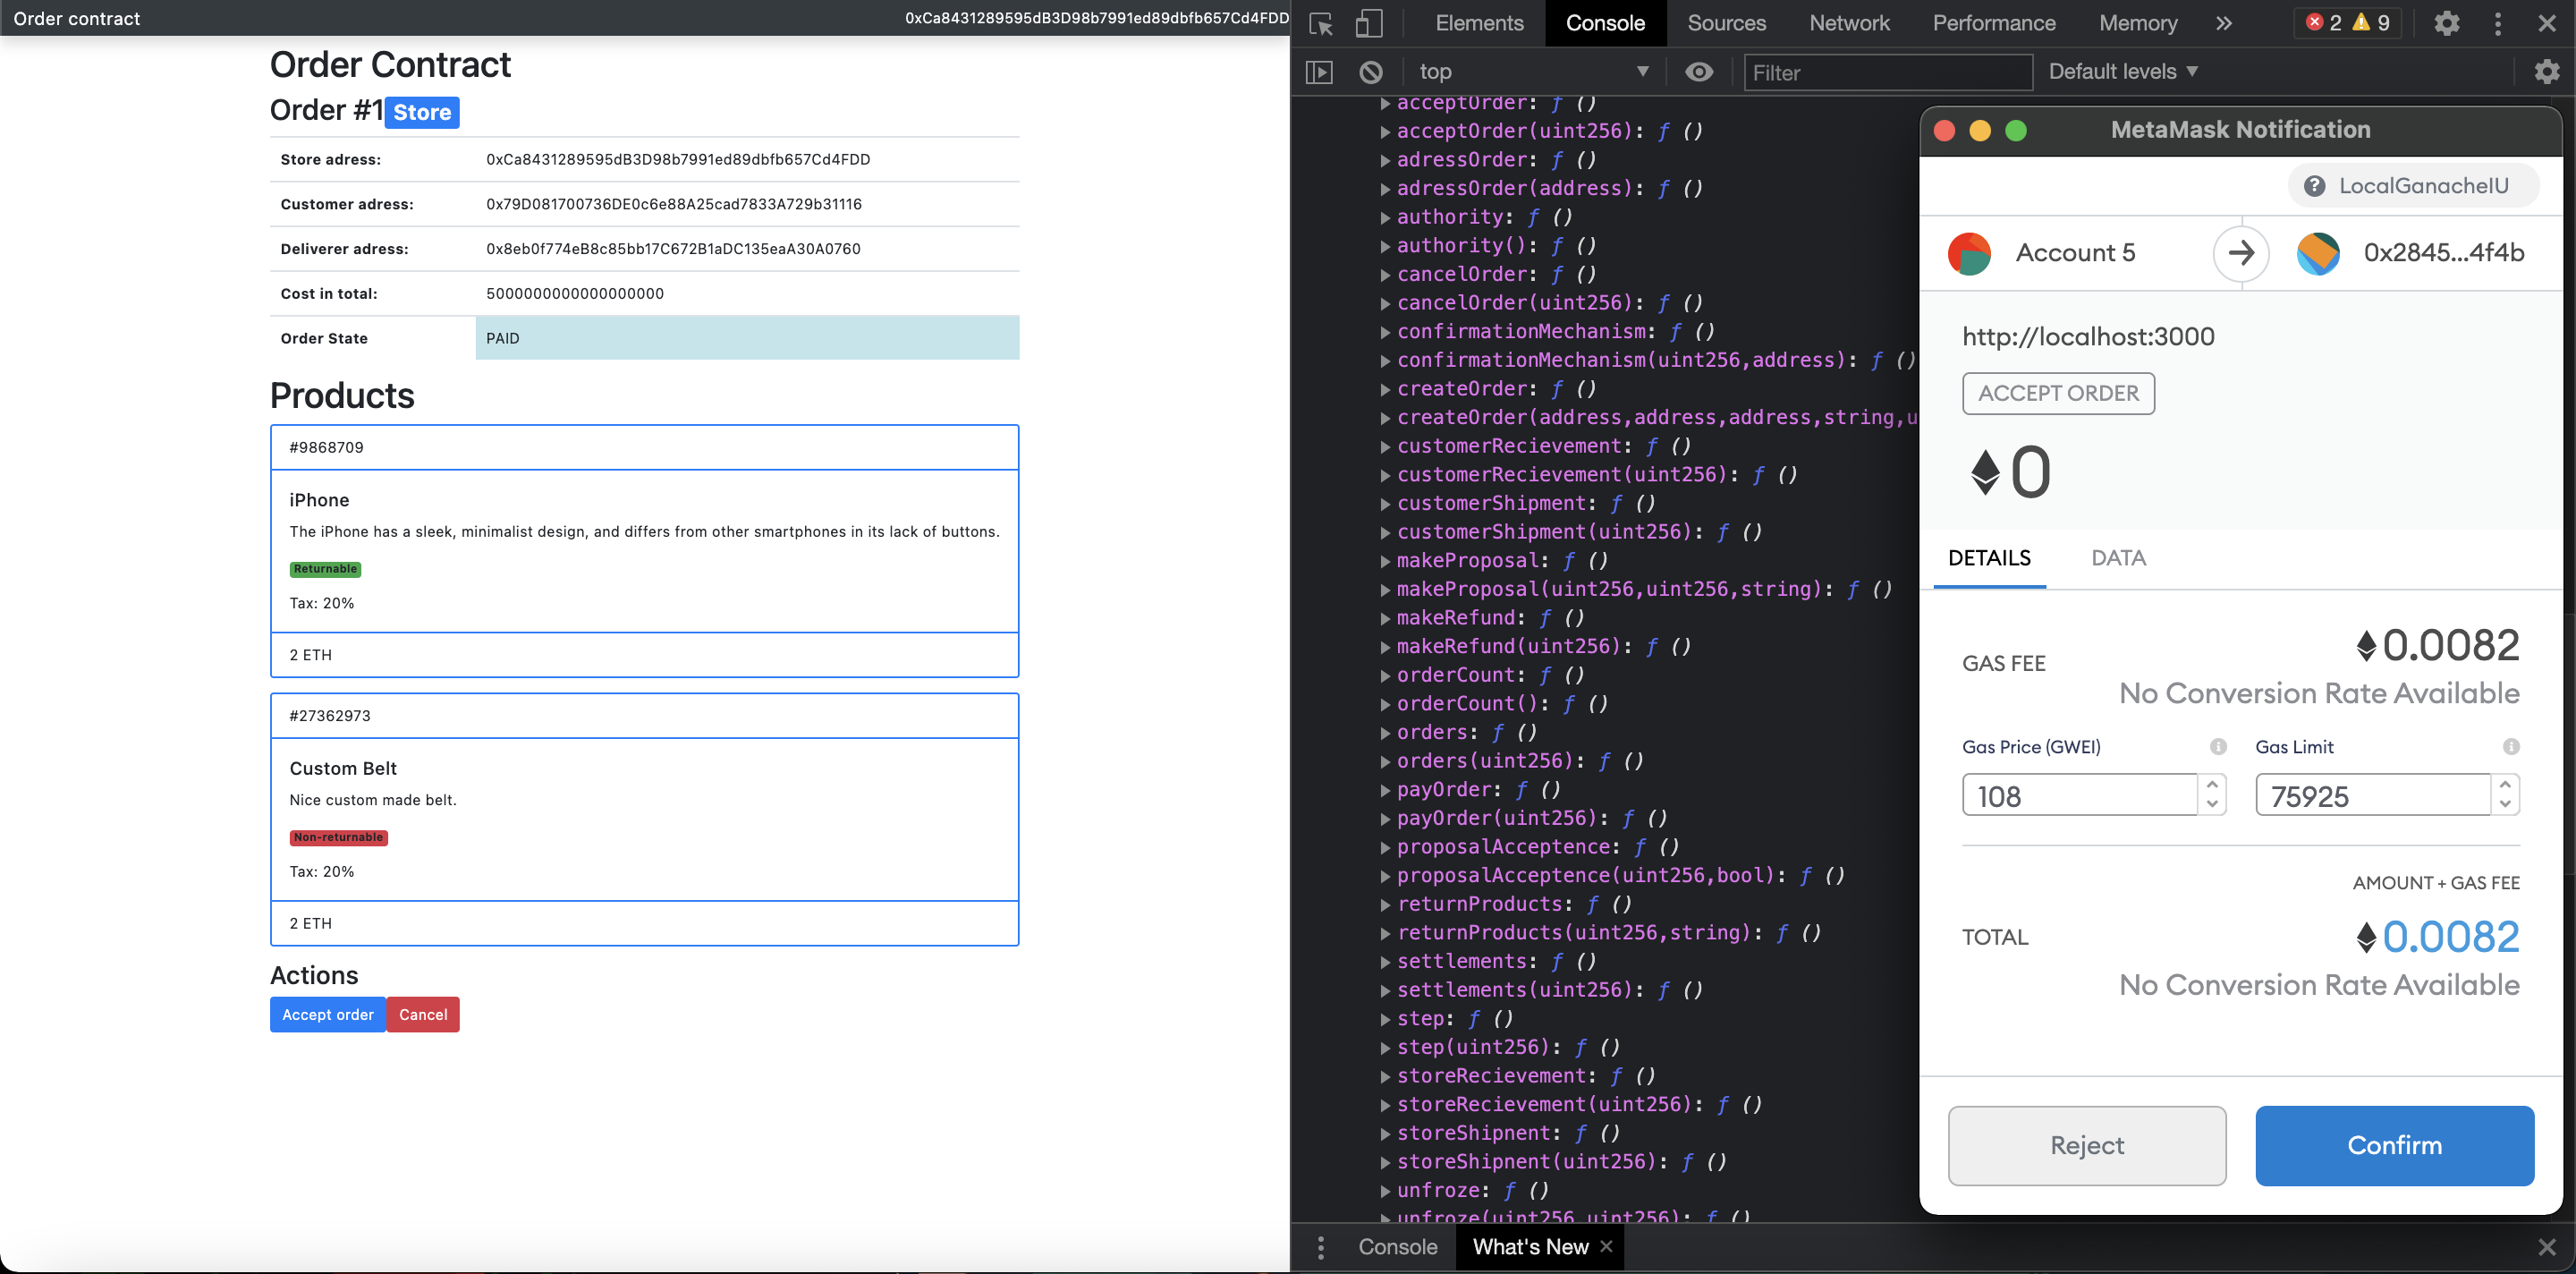
\includegraphics[width=\textwidth]{assets/Screenshot 2021-04-17 at 16.10.29.png}
    \caption{Proof of concept screen with console (all screens: EA8) }
    \label{fig:screenProofOfConcept}
\end{figure}


\subsection{Code example}

Application is written in Javascript with the React.js framework and Web3.js library for communication with a smart contract. The mandatory part for interacting with the application is a cryptocurrency wallet (we recommend Metamask). The application is not for a standalone use, so it needs a predefined API provided by the store. This is not a problem because the purpose of the application is to be packed in a plugin for online store solutions, so the plugin can expose its own API, so compatibility is guaranteed. For a proof of concept use, we have created \texttt{StoreAPI.js} to simulate the plugin API.

Web3.js handles the essential part of the functionality: sending the transactions and subscribing to the smart contract event \texttt{OrderStateChanged}. Now follows tiny examples of the code to understand the functionality, with the situation, you are in Store role, and a new paid order came. 

\begin{minipage}{\linewidth}
\begin{lstlisting}[caption=OrderLogicContract.sol getOrder function]
    async getOrder(){
      if ( this.state.orderFromStoreInfo.id !== undefined ){
        // Web3.js call to orderLocgic contract to get actual order informations
        const order = await this.state.orderLogic.methods.orders(this.state.orderFromStoreInfo.id).call()
        this.setState({ order  : order })
        this.setState( { orderState : OrderState.getName(order.state) } )
        this.determineRole() // Set role based on loged user and order info
        this.watchOrderEvents() // Start watching OrderStateChanged events
        ...
    }

\end{lstlisting}
\end{minipage}

Now we know all the stored order's information from the local Ethereum network. We can set this information to the global state of the application's reactive components can reflect a changed state. In our case, this code will react and will show the store relevant action buttons. 

\begin{lstlisting}[caption= App.js react JSX aviable actions ]
{ (this.state.orderState === OrderState.PAID &&
   this.state.role === Role.STORE )  &&
  <p>
    <button type="button" className="btn btn-primary" onClick={this.acceptOrder}>Accept order</button>
    <button type="button" className="btn btn-danger" onClick={this.cancelOrder}>Cancel</button>
  </p>
}

\end{lstlisting}

Clicking on the accept order button will trigger the \texttt{acceptOrder function} and a transaction call will be created. 

\begin{lstlisting}[caption=App.js calling acceptOrder function on smart contract]
 async acceptOrder(){
    this.state.orderLogic.methods.acceptOrder( this.state.order.id).send(
        {from: this.state.account}).once( 'receipt', (receipt)  => {
            ... // code
    })
  }
\end{lstlisting}

The last example is from the watch function. By calling \texttt{acceptOrder} the order changes its state and the \texttt{OrderStateChanged} will be emitted. This code is listening to these events. When we received the order change, we can react to it and change the application's state. 

\begin{lstlisting}[caption=App.js receiving OrderStateChanged events]
watchOrderEvents(){
  this.state.orderLogic.events.OrderStateChanged({})
      .on('data', event => {
        if ( this.state.order !== null ){ // fix for creating one
          if ( event.returnValues.orderId === this.state.order.id ){
             this.getOrder()
          }
        }
      })
}
\end{lstlisting}


\subsection{Communication example}

Now, we have an overview of how frontend and backend parts work, so it is time to describe its communication. Figure \ref{fig:sekvencialFlow} shows the sequential flow between the user application and two contracts. The first transaction is only between the application and one contract, where a confirmation is created. The second transaction is more complicated, because the \texttt{OrderlogicContract} has another call to \texttt{DeliveryContract} to confirm the delivery act.  The code example of this call is in listing \ref{lst:comfirmationMechanismExample}.

It is necessary to mention that \texttt{function isConfirmed( uint \_orderId, address consigor, address recipient ) public view returns ( bool eval )}  is a view function, so there is no additional gas consumption for calling this method because it is not changing the state of the \texttt{DeliveryContract}. 

\begin{figure}[ht!]
    \centering
    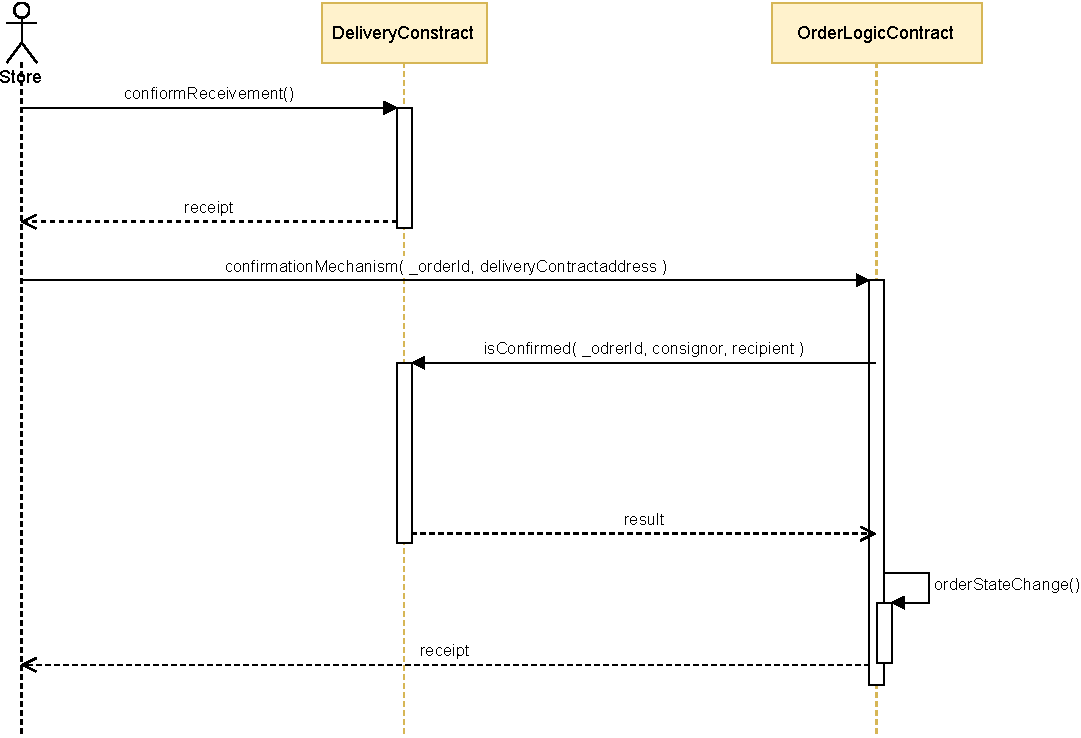
\includegraphics[width=\textwidth]{assets/SequenceDiagram.pdf}
    \caption{Sequence diagram of contract communication}
    \label{fig:sekvencialFlow}
\end{figure}


\section{Testing of the proof of concept}

We face a complicated contract with immense responsibility, so it is necessary to be as safe as possible, with zero tolerance to bugs. Of course, our proof of concept doesn't include the safest implementation, but to provide some safety and bug catching, we have created a test set, which tests the contract's most common scenarios. The code example below shows the testing of Accept state role. We can see, that only the store address is able to call the \texttt{acceptOrder function} and after call, we are testing the change of the order's state.

\begin{minipage}{\linewidth}
\begin{lstlisting}[caption=OrderLogicContract.js test case of Accept state]
it('Accept state', async () => {
    orderContract.acceptOrder(orderCount, {from: authority}).should.be.rejected;
    orderContract.acceptOrder(orderCount, {from: customer}).should.be.rejected;
    orderContract.acceptOrder(orderCount, {from: deliverer}).should.be.rejected;
    orderContract.acceptOrder(orderCount, {from: store}).should.be.ok;
    const order = await orderContract.orders( orderCount )
    assert.equal(order.state.toNumber(), 2, 'Accept is ok')
})
\end{lstlisting}
\end{minipage}

The second example is testing the claim of the store payment. We are using \texttt{notStrictEqual} method because the difference of balances before and after will be not exactly \texttt{totalOrderConst}, but less. It is because of the fee for calling \texttt{.step} function. In the end, we are testing the change of the order's state.


\begin{lstlisting}[caption==OrderLogicContract.js test case of Claim payment]
it('Claim payment', async () => {
    let amountBefore = await web3.eth.getBalance( store );
    amountBefore = new web3.utils.BN(amountBefore);

    await orderContract.step( orderCount,  {from: store} );

    let amountAfter = await web3.eth.getBalance( store );
    amountAfter = new web3.utils.BN(amountAfter);

    const order = await orderContract.orders( orderCount )
    let toAdd  = web3.utils.toWei(orderCost, 'Ether')

    const exepectedBalance = amountBefore.add( new web3.utils.BN(toAdd) )
    // No strict for gas expences
    assert.notStrictEqual(amountAfter.toString(), exepectedBalance.toString())
    assert.equal(order.state.toNumber(), 6, 'Claim Payment is ok')
})
\end{lstlisting}



We have created 37 test sets for the most common ways of the order process. The tests are for delivery deployment (1 set), confirmation mechanism (4 sets), order deployment (2 sets), successful order (6 sets), returned order (9 sets) , authority resolving (10 sets) and order cancellation (5 sets). They provide nice examples of how the contract should work.

\section{Chapter summary}
This chapter described the implementation principle of the described system. We had a walkthrough of used technologies, implementation and architecture of the \texttt{OrderLogicContract} and Delivery contract. We have looked at how the frontend application works and how to reflect changes based on the smart contract state, thanks to emitting events. We have introduced the example of testing the smart contract and with implementation examples.

Now you should have an idea of how the whole system can be implemented and what problems can occur during the project. By creating this proof of concept, we have a useful tool for measuring the transactions' approximate cost, which we can use to look at the system from a business perspective in the next chapter.


\chapter{Evaluation}
% Evaluation
% Business use
Business is an uncompromising world with zero tolerance for failure. If some product or technology should have a chance to be successful in the business world, it has to have business potential. This chapter discusses the business advantages and dilemmas of blockchain intermediary solution for online orders. 

We will estimate the costs efficiency of the smart contract solution and then we compare these results with a Paypal solution. We don't stop only with cost comparison, but we will look at the security, transparency and scalability. 

\section{Cost efficiency}


% Future improvements
We connect to the previous chapter \ref{proofOfConcept}, and use created proof of concept to get estimated metrics of the system. The proof of concept is not optimized for gas consumption or storage efficiency, but for this thesis is an excellent tool for getting relevant data. The final system will not be radically different.

\subsection{Proof of concept metrics}

The first thing that we can mine from proof of concept is a gas consumption. We have measured the gas consumption of each order transaction and the deployment of smart contracts. The contract is designed to be deployed only once, and the store, deliverer or the customer does not pay this fee.  
 
The second parameter that we need is the average gas price for a unit. We use the Etherscan website to get this parameter. At the time of making this calculation, the average gas unit price ws set to 108 GWei.

Finally, to recalculate the fee to fiat currency, we need to have a conversion rate. The conversion rate between ETH and EUR is 1ETH = 1982,82EUR (17. 4., 18:35 UTC from \href{https://www.coinbase.com}{Coinbase}). This rate is changing rapidly, so today this rate is probably a lot different. 

Look at the table of measured values in external attachments EA5. In figure \ref{fig:gasSpend} you can see the graph of measured values. 


\begin{figure}[ht!]
    \centering
    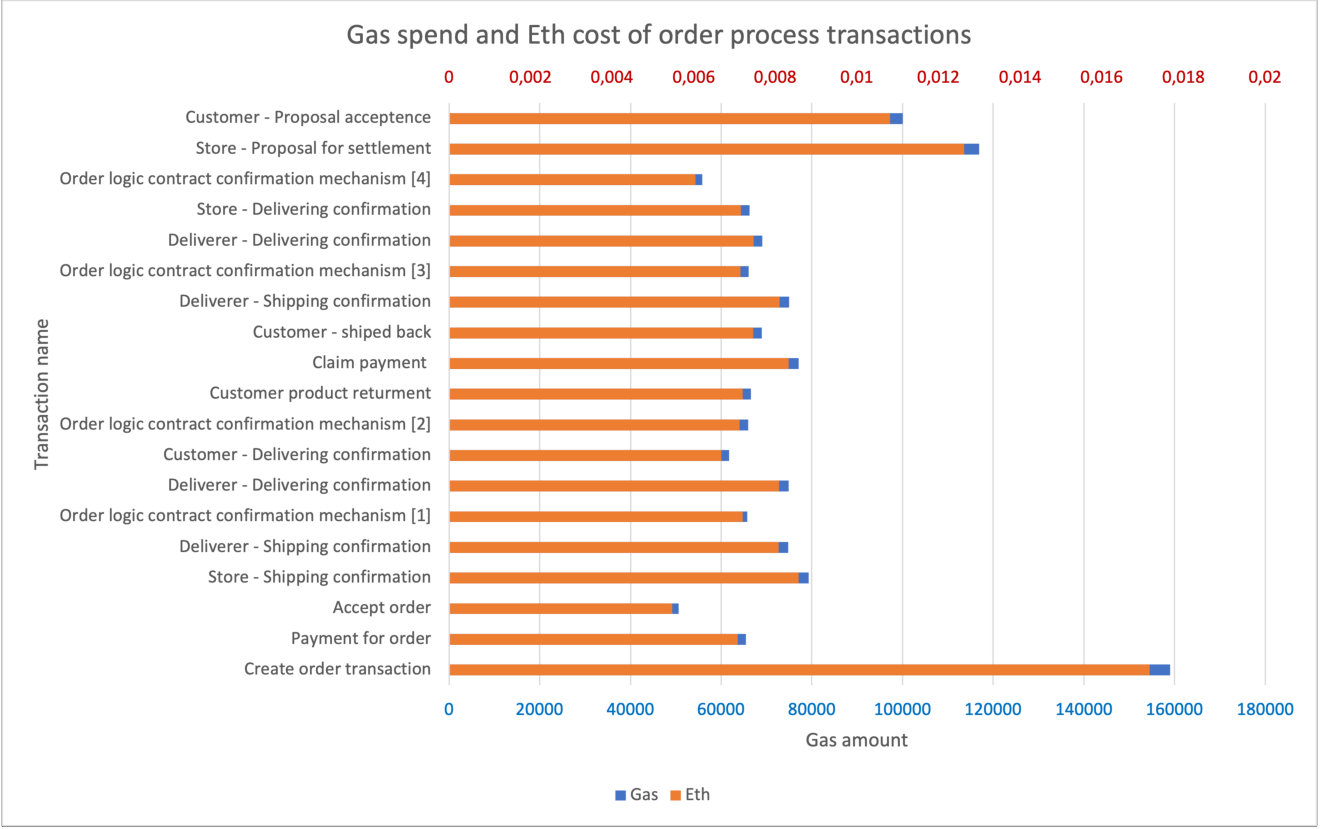
\includegraphics[width=\textwidth]{assets/PoCMetrics3.pdf}
    \caption{Gas spent and ETH cost of order processing transactions (data: EA5)}
    \label{fig:gasSpend}
\end{figure}


Altogether, the price for one entire process walkthrough is 0,149378 ETH what is an astronomical price of 296 EUR. That is an enormous price for an intermediary, isn't it? Of course, with this price point, there is no chance to use these contracts nowadays. Before we throw this idea into a trash, let's look at what influences the final price for the contract and some ways how to reduce it.

\subsection{Influences and reductions of the costs}

The final price consists of three parts: the amount of gas spent, the price for a gas unit and the conversion rate. Now we take a closer look at each of them.

\begin{description}

\item[The gas spent] is influenced by computing steps, data transfers and memory use. Existing techniques to write a solidity code optimize for gas spent. Mostly the unnecessary expenses come from cycles or dead code. We are also not storing the whole strings of products, only hashes for this reason. We are losing the information of concentrate products, but we can still evaluate the correctness of the order. 


\item[Price for a gas unit] works on standard economic principle. The price for a gas unit depends on the ratio of waiting transactions and the number of miners. Now this ratio is extremely bad for users and developers, but lucky times for miners.  For the designed process, the opposite state or balanced state of the network is beneficial. \cite{gasHigh}

A future update of the Ethereum network from Proof of Work to Proof of Stake can dramatically reduce the transaction costs.

\item[The conversion rate] has extremely high volatility nowadays. Sadly, we can't predict the movement.

\end{description}



\section{Comparison with other solutions}

We have used the Paypal solution as inspiration and intermediary a lot, now it is time to compare these two solutions not only from price perspective. By the price table from their official website \cite{paypalfees}, here is a small graph example in figure \ref{fig:PaypalFees}. The dispute fee can be charged based on the Paypal decision or even can be assigned a high volume dispute fee. The table \ref{fig:PaypalFees} is counting with a standard dispute fees. 

\begin{figure}[ht!]
    \centering
    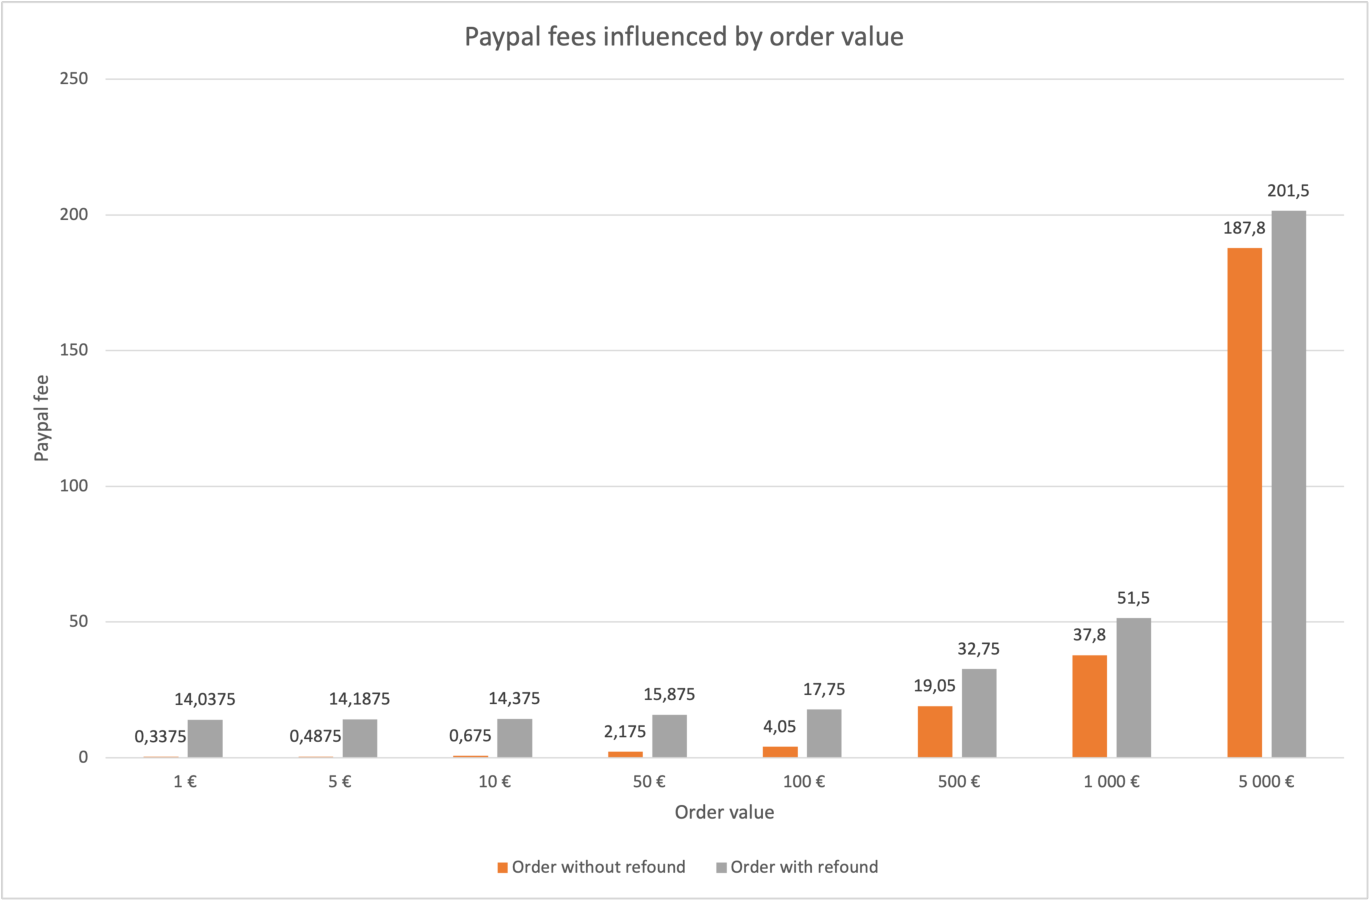
\includegraphics[width=\textwidth]{assets/PaypalFees.pdf}
    \caption{Paypal fees influenced by order value  (data: EA5)}
    \label{fig:PaypalFees}
\end{figure}




On the other hand, the smart contract solution has almost constant fee for all orders. The process ended in a refunded state is naturally more expensive than finished in a complete state, but the price of the order does not influence the final price. 

The table \ref{comparisionOfSolutions} compares a smart contract solution, Utrust solution and Paypal service from a different point of views. Utrust is also an intermediary prototype of the solution, which works with cryptocurrency, but there is no smart contract on the backend, but their own systems. \cite{utrust}


\begin{table}[ht!]
\caption{Comparison of payment solutions} \label{comparisionOfSolutions}
\begin{tabular}{| p{2cm} | p{3cm} | p{3cm} | p{3cm} | }
\hline
Field &
  Paypal &
  Utrust &
  To-be model \\ \hline
Fees &
  0.30€ + 3,75\% from order price &
  1\% from order price &
  Constan fee based on nubder of transactions \\ \hline
Data &
  Data are stored in Paypal servers, which full copy of the order &
  Data are stored in Utriust servers (not mode specified) &
  Hashes of data are store in public network \\ \hline
Pesonal data &
  Users has an Paypal account &
  Users has an Utrust account &
  Possibility to suppor virtial identity \\ \hline
Supported currency &
  Fiat currencies (USD, EUR, RUB ...) &
  Payment in crypto (Ethereum, Bitcoun, Utrust) and convertions to fiat currencies (USD, EUR, RUB ...) &
  Only crypto (Ethereum) \\ \hline
Supported solution &
  In-call support, e-mail support, account onpen a dispute posability &
  Forum support, account open a dispute &
  No support, only a blochchain arbitration or authority help in frozen state \\ \hline
Supported e-commerce solutions &
  Woocommerce, Magento, PrestaShop, Utust API, JumpSeller, OpenCart, Payrexx, Shopify .... &
  Woocommerce, Magento, PrestaShop, Utust API, JumpSeller, OpenCart, Payrexx, Shopify &
  Posibility to support all solutions \\ \hline
\end{tabular}
\end{table}

After this validation, it does not look well with the idea of using a smart contract as an intermediary for online payments. And that is completely fine because blockchain is only at the beginning, and the more popular blockchain is, the better the smart contract solutions become. 

\section{Benefits and impacts of the to-be state}

To truly understand the potential of this solution, we need to go further in time. We need to imagine how the world can use blockchain technology, and smart contract payment will be only one piece of the puzzle in the whole image. We mentioned a few benefits of blockchain use earlier in \ref{blockchainInEcommerce}, so now we look at "How smart contract order payments can improve blockchain idea". We will also continue from the idea of an advanced future architecture described in \ref{advancedFutureArchitecture}.

\begin{description}
    
\item[Supply chain management:] The to-be model is specially designed to support third party delivery contract. The only restriction is to conform the delivery contract interface with one mandatory function. So the delivery contract (or contracts) can do much more. Promising function candidates are to calculate prices or the traceability for end-user functions. Would not it be perfect to see where the goods come from directly on the website? Or to evaluate the originality of ordered goods. Every aspect of the delivery contract depends on the deliverers and stores. 

\item[Fraud reduction:] Using the to-be model will make scam at the stores a lot harder. It is exponentially harder to scam someone when everything you do is immutably written into blockchain. On the other side, if people are not well informed about how to interact with a contract, there is always a way how to scam them. It will require a lot of time and energy to teach people that they are fully responsible for their decisions, and there is no step back function in blockchain.

It can't be an automatically safe operation to "pay by crypto protected by smart contract" and the customers have to be careful where they are sending a transaction. They have to pay attention if they are signing a transaction for the right smart contract. In future, it can be a useful tool to check this information for users as now web browsers are checking the certificates of web sites, but as you know it's not 100\%.

\item[Marketing and reviews:] Online reviews are the basic pillar of public opinion. We have talked a lot about reviews and their verification in \ref{reviews}. The to-be model can serve as a fantastic example of review verification, where the reviewer can review only the order, that they made, and the public sees what really happened. The potential customer can see not only the ratio of satisfied customers but also the number or successfully completed orders. It will become much easier to estimate the store's credibility.

\item[Protecting personal information and privacy:] To-be model is opened to support virtual identities. There is no requirement that the customer address has to be an externally owned account. It can be freely a smart contract with an interface for providing proofs (proof of age as an example) as verifications to order logic contract. 

We can go even further, and the stores can also have their validators, so the store account doesn't have to be EOA account and can be linked to a public registration entity. 

\item[Scalability:]  Designed to-be model is ready for having a variety of logics for specific geolocation law restrictions. It is almost impossible to have one order logic for all countries. As indicated, the official order logic contract will be created by the government authority to respect local laws and enable law forces to interfere with transactions (in a frozen state as decision authority of course).

\item[Cost reduction:] We have talked, that this kind of solution has the advantage of the constant cost fee for transactions. Ethereum in not only working blockchain and in the future other cheaper solutions can become popular. We have used Das contract methodology and it is not fixed to Ethereum. The working principles can be used in others blockchains as well.  

\end{description}

Besides these benefits, some challenges have to be solved. Blockchain is a relatively new technology and people have to learn how to interact with it. They have to understand what it means, that the transactions are public. A huge challenge will be for humanity to trust the blockchain technology.

Blockchain brings responsibility to users, so they are responsible for every signed transaction. Only the user is responsible for their secret key and the seed phase. If the user is not careful enough, it can easily lead to a loss of their crypto coins and no one would be able to help them.


\section{Chapter summary}
We talked about the cost efficiency of designed to-be models and compared this model with Paypal and Utrust solutions. The to-be model is not well suited for today's use (mainly for transaction costs), but it has promising benefits and advantages in future.

We have also described the impact of the to-be model on the eCommerce market from different perspectives and which challenges blockchain technology can expect in future to become successful.




\chapter{Conclusion}



This diploma thesis shows that blockchain technology has the potential to change eCommerce, to help legitimate sellers and fair customers.

The beginning of this work was devoted to introducing and explaining the basic principles and ideas of blockchain and its specific implementation in the form of Ethereum. Understanding how Ethereum works is the key to a deeper understanding of Smart Contracts and their purpose. The end of the chapter is dedicated to BPMN and its symbols, which helped us understand the modelled processes.

The third chapter introduced the world of eCommerce and its essential pillars. It informed about the technical possibilities of modern online stores and fundamental processes such as payments and delivery. Great attention was paid to the purchase contract because the whole logic of the designed model is based on it. The end of the chapter describes the inspiring use of blockchain in the eCommerce sphere.

The analytical part examines in detail the order process in the online store and reveals existing solutions. From the analysis follows buyers protection in online payment process is a critical need. This fact has a significant impact on the creation of a to-be model using smart contracts. The system is based on non-functional and functional requirements, which are developed into use cases. This knowledge is the heart of the technological architecture of the system.

As for verifying the feasibility of the proposed to-be solution, we implemented a proof of concept. As proof of concept, a decentralized application has been created. User can log in using a crypto wallet and interact with blockchain network. DApp handles the entire communication part of the system with smart contracts. There are two smart contracts in the network that interact with each other. The first takes care of the order logic and the second is used to support delivery.

The end of the work pays attention to the use of this solution in the real world. It deals with the proposed model from a business and financial point of view and the conditions that affect it. It focuses on the benefits and impacts of the solution.

The work introduced a new concept of how online orders can work and discussed its feasibility in the future. Blockchain is just beginning its journey, and we believe that this work will help to develop it, not only in terms of technology, but also in bringing it closer to the public.

This thesis brings insights for further research.

\begin{itemize}
\item Extend the to-be model to work with Decentralized identity
\item Experiment to use different blockchain technologies
\item Recreate the to-be model for other countries, with their law specifics
\item Implement the blockchain-based review mechanism for the completed orders with statistics about customers and sellers
\item Implement the browser extension for validation of trusted smart contracts
\item Compare the possibilities of different implementations of delivery contract, with support of presented model
\end{itemize}




%\bibliographystyle{iso690}
%\bibliography{ref}

\printbibliography


\setsecnumdepth{all}
\appendix

\chapter{Acronyms}
% \printglossaries
\begin{description}
    \item[BPMN] Business Process Model and Notation
    \item[CA]   Contract account
    \item[dApp] Decentralized Application
    \item[DAO]  Decentralized Autonomous Organization
    \item[DID]  Decentralized identifier
    \item[EA]  External attachment
    \item[EVM]  Ethereum Virtual Machine
    \item[EOA]  Externally owned account
    \item[ETH]  Ethereum currency
    \item[GDPR] General Data Protection Regulation
	\item[PoS]  Proof of Stake
	\item[PoW]  Proof of Work
    \item[SAAS] Software as a service
\end{description}


\chapter{Contents of enclosed USB}

%change appropriately

\begin{figure}
	\dirtree{%
		.1 readme.md\DTcomment{the file with contents description}.
		.1 external attachments\DTcomment{directory with external attachments}.
		.2 EA1 As-is model.
		.2 EA2 To-be model.
		.2 EA3 Requiretements and use-cases.
		.2 EA4 DasContract to-be model.
		.2 EA5 PoCMetricts.
		.2 EA6 ThesisShowcase.
		.2 EA7 code.
		.2 EA8 process simulation.
		.2 EA9 Diagrams.
		.1 src\DTcomment{the directory whole dApp}.
		.2 migrations\DTcomment{migration files}.
		.2 src \DTcomment{source code of the dApp}.
		.3 components\DTcomment{react application}.
		.3 contracts\DTcomment{smart contract source code}.
		.2 test \DTcomment{tests for the application}.
		.1 text \DTcomment{the thesis text directory}.
		.2 thesis.pdf \DTcomment{the thesis text in PDF format}.
		.2 thesis \DTcomment{the directory of \LaTeX{} source codes of the thesis}.
		.1 LICENSE \DTcomment{License file}.
	}
\end{figure}

\end{document}
